%------------------氯化聚氯乙烯的热稳定和润滑体系研究-----------------%
%----------------------------朱浩南-----------------------------%

%---------------------------定义文档类型-------------------------%
%   \documentclass[param]{class}
%   param{
%       a4paper: A4纸
%       oneside: 单面打印
%       onecolumn: 单列排版
%       12pt: 默认字体大小
%   }
%   class{
%       report: 长报告、论文
%       article: 短文章
%       ctexrep: ctex report
%---------------------------------------------------------------%
    
\documentclass[a4paper, twoside, onecolumn, notitlepage, 12pt]{ctexrep}    % transmag 实现双列排版,摘要跨列
% titlepage 标题单独分页 notitlepage 标题不单独分页

%----------------------------引入宏包---------------------------%
\usepackage[utf8]{inputenc} %特殊符号
%\usepackage{xeCJK}      %CJK引擎,使用 CTex 文档类后不再需要次宏包
%\usepackage{abstract}  %摘要与关键词
\usepackage{graphicx}   %插图工具包
\usepackage[super, square]{natbib}     %漂亮的bib引用    super-上标, square-方括号
\usepackage{bm}         %设置缩进
\usepackage{fancyhdr}   %定制页眉页脚
\usepackage{chemfig}    %化学方程式
\usepackage{amsmath}    %数学公式阵列
\usepackage{multirow}   %表格合并单元格
\usepackage{setspace}   %行距宏包
\usepackage{geometry}   %页边距宏包
\usepackage{fontspec}   %字体
\usepackage{enumerate}  %定制列表序号样式
\usepackage{makecell}   %表格内容换行
\usepackage{pifont}     %实现带圈数字,①开始于\ding{192}
\usepackage[perpage,symbol*]{footmisc}
\usepackage[justification=centering]{caption}   %标题设置
\usepackage{float}      %设定图片的位置    \[H]可固定图片位置
\usepackage{tikz}       %tikz图形库
\usepackage{flafter}	%防止图表出现在引述文字之前
\usepackage{tabularx}


%----------------------------设置字体族--------------------------%
%\CJKfamily{SimSun}
\setmainfont{Times New Roman}
\setsansfont{Arial}
\setmonofont{Noto Mono}
\setCJKmainfont[BoldFont=SimHei]{SimSun}

%\newcommand{\song}{\CJKfamily{simsun}}  % 宋体
\newcommand{\hei}{\CJKfamily{SimHei}}   % 黑体


%------------------------------设置字体大小------------------------%  
\newcommand{\chuhao}{\fontsize{42pt}{\baselineskip}\selectfont}     %初号  
\newcommand{\xiaochuhao}{\fontsize{36pt}{\baselineskip}\selectfont} %小初号  
\newcommand{\yihao}{\fontsize{28pt}{\baselineskip}\selectfont}      %一号  
\newcommand{\erhao}{\fontsize{21pt}{\baselineskip}\selectfont}      %二号  
\newcommand{\xiaoerhao}{\fontsize{18pt}{\baselineskip}\selectfont}  %小二号  
\newcommand{\sanhao}{\fontsize{15.75pt}{\baselineskip}\selectfont}  %三号  
\newcommand{\sihao}{\fontsize{14pt}{\baselineskip}\selectfont}      %四号  
\newcommand{\xiaosihao}{\fontsize{12pt}{\baselineskip}\selectfont}  %小四号  
\newcommand{\wuhao}{\fontsize{10.5pt}{\baselineskip}\selectfont}    %五号  
\newcommand{\xiaowuhao}{\fontsize{9pt}{\baselineskip}\selectfont}   %小五号  
\newcommand{\liuhao}{\fontsize{7.875pt}{\baselineskip}\selectfont}  %六号  
\newcommand{\qihao}{\fontsize{5.25pt}{\baselineskip}\selectfont}    %七号

%------------------------------设置标题样式-------------------------------%
%\renewcommand{\contentsname}{目录}  % 将Contents改为目录
%\renewcommand{\abstractname}{摘要}  % 将Abstract改为摘要
%\renewcommand{\refname}{参考文献}   % 将References改为参考文献
%\renewcommand{\indexname}{索引}
%\renewcommand{\figurename}{图}
%\renewcommand{\tablename}{表}
%\renewcommand{\appendixname}{附录}

\setcounter{secnumdepth}{3} %设置编号深度
%\renewcommand{\thepart}{\textbf{第\arabic{part}部分}}
\renewcommand{\thesection}{第\arabic{chapter}. \arabic{section}节}
\renewcommand{\thesubsection}{\arabic{chapter}. \arabic{section}. \arabic{subsection}}
\renewcommand{\thesubsubsection}{\arabic{chapter}. \arabic{section}. \arabic{subsection}. \arabic{subsubsection}}


% 实现带圈脚注样式
\DefineFNsymbols{circled}{{\ding{182}}{\ding{183}}{\ding{184}}
{\ding{185}}{\ding{186}}{\ding{187}}{\ding{188}}{\ding{189}}{\ding{190}}{\ding{191}}}
\setfnsymbol{circled}

% 设置小写字母脚注样式
%\renewcommand{\thefootnote}{\alph{footnote}}


%-------------------------------设置间距属性-----------------------------%
\usepackage{indentfirst}
\setlength{\parindent}{2em} %设置自动缩进为两格
\setlength{\baselineskip}{22pt}    %设置行距
% \renewcommand{\baselinestretch}{1.2}   %设置 1.2 倍行距
% \linespread{1.2}            %设置 1.2 倍行距
\geometry{left=2.7cm, right=2.7cm, top=3.5cm, bottom=2.6cm} %设置页边距
\setlength{\itemsep}{0pt}   %设置列表元素间距
\setlength{\parskip}{0pt}  %设置段间距
\CTEXsetup[beforeskip={0pt}]{chapter}	%章节前不留空白
\captionsetup{font={small}}				%设置图表标题大小
\setlength{\abovecaptionskip}{-0pt}		%图表标题与图标间距
% \setlength{\bibsep}{5pt}				%参考文献间距


%-------------------------------设置数学环境-----------------------------%
\setatomsep{2em}    %设置全局化学键长度

%设置高分子的括号
\newcommand\setpolymerdelim[2]{\def\delimleft{#1}\def\delimright{#2}}
\def\makebraces[#1,#2]#3#4#5{%
\edef\delimhalfdim{\the\dimexpr(#1+#2)/2}%
\edef\delimvshift{\the\dimexpr(#1-#2)/2}%
\chemmove{%
\node[at=(#4),yshift=(\delimvshift)]
{$\left\delimleft\vrule height\delimhalfdim depth\delimhalfdim
width0pt\right.$};%
\node[at=(#5),yshift=(\delimvshift)]
{$\left.\vrule height\delimhalfdim depth\delimhalfdim
width0pt\right\delimright_{\rlap{$\scriptstyle#3$}}$};}}
\setpolymerdelim[]

%   调用时使用类似以下的命令
%   \setpolymerdelim[]  设定括号样式,若为圆括号则()
%   \chemfig{-[@{op,.75}]CH=CH-\lewis{2.,C}H-CH_2-[@{cl,.25}]}  此处.75  .25两个参数分别为两个化学键在括号左边部分的比例
%   \makebraces[5pt,5pt]{}{op}{cl}  此处 5pt 为两个括号的大小

% 引用 tikz 装饰库,用于绘制波浪形键
\usetikzlibrary{decorations.pathmorphing}

% 定义矩形框
\usetikzlibrary{shapes.geometric, arrows}
\tikzstyle{pro} = [rectangle, minimum width = 3cm, minimum height = 1cm, text centered, text width = 3cm, draw = black]
\tikzstyle{io} = [rectangle, rounded corners, minimum width = 3cm, minimum height = 1cm, text centered, text width = 3cm, draw = black]

\tikzstyle{arrow} = [, ->, >= stealth]
\tikzstyle{line} = [, -, >= stealth]


%-------------------------------设置快捷命令-----------------------------%
\newcommand{\cd}{$^{\circ}$C}  %摄氏度
\newcommand{\va}{\vphantom}         %使第一个化学键居中
\newcommand{\borderLine}{\Xhline{1pt}}	%设置表格边界线命令
\newcommand{\interLine}{\Xhline{0.5pt}}		%设置表格分隔线命令
\newcommand{\mc}{\makecell[c]}



%--------------------------------添加页面元素----------------------------%
\title{\sanhao \textbf{氯化聚氯乙烯热稳定和润滑体系研究}\vspace{-8ex}}
% \author{
%     \wuhao 朱浩南,高材1314,2013012433\\
%     \wuhao 指导教师:武德珍,教授
% }
\date{}

%设置页眉页脚
\fancyhf{}
\pagestyle{fancy}
\lhead{\xiaowuhao \leftmark}    %显示章节标题
\chead{\xiaowuhao 北京化工大学毕业设计(论文)}
\fancyfoot[C]{\thepage}
%设置双下划线页眉
\makeatletter %双线页眉
\def\headrule{{\if@fancyplain\let\headrulewidth\plainheadrulewidth\fi%
\hrule\@height 1.0pt \@width\headwidth\vskip1pt%上面线为1pt粗
\hrule\@height 0.5pt\@width\headwidth  %下面0.5pt粗
\vskip-2\headrulewidth\vskip-1pt}      %两条线的距离1pt
\vspace{6mm}}     %双线与下面正文之间的垂直间距
\makeatother

%-------------------------------文档部分---------------------------------%
\begin{document}

\pagestyle{fancy}
\pagenumbering{Roman}
\setcounter{page}{1}

\maketitle

\begin{abstract}\xiaosihao
    氯化聚氯乙烯(CPVC)的热稳定性差,熔体黏度高,加工时易发生热分解脱氯化氢,因此需要在 CPVC 加工过程中加入热稳定剂和润滑剂。润滑剂是 CPVC 加工过程中不可缺少的一类加工助剂,但润滑剂的加入会对材料的力学性能产生一定的影响。因此在本实验的第一部分对不同类型的外润滑剂进行了研究,通过热性能和力学性能来寻找相同加入量下润滑效果最好的外润滑剂。\par
    长期以来,铅盐类热稳定剂被作为热稳定剂的首选使用,但随着人们对铅污染的认识加深,铅盐类热稳定剂逐渐被其他类型的热稳定剂替代。如有机锡热稳定剂因其稳定效果好、污染小的特点,正逐渐成为 CPVC 加工过程中的稳定剂选择。但由于有机锡的价格相对较高,使其的应用发展受到了限制。因此本实验的第二部分正是研究不同型号和种类的有机锡热稳定剂的热性能和力学性能,从而找到在相同用量下能提供较好热稳定性的有机锡品种。\par
    为寻找润滑效果最好的外润滑剂,本文对 AC-316、AC-617、AC-629 和 PEW-0380 四种外润滑剂进行了静态热稳定性、动态热稳定性、力学性能以及动态力学热分析的测试。研究发现,AC-629 与 PEW-0380 能提供较好的润滑效果和塑化效果;但在较高温度下,由于 AC-617 与 AC-629 的滴点较低,使得润滑剂提前失效,润滑效果反而下降;在四种外润滑剂中,PEW-0380 能使 CPVC 提供最好冲击强度。在本实验的第二部分,对 TMG-234、T-190A 和液体有机锡 3 种有机锡热稳定剂进行了测试。研究结果表明,液体有机锡能提供较好的热稳定性,但其长期热稳定性较差且热稳定时间短,同时其对 CPVC 的强度和韧性的损失较小;T-190A 对 CPVC 的硬度损失较小。\par
    \textbf{关键词:氯化聚氯乙烯;热稳定剂;润滑剂;有机锡;聚乙烯蜡}
\end{abstract}

\renewcommand\abstractname{Abstract}
\clearpage
\begin{center}
	\sanhao \textbf{Study on Thermal Stability and Lubrication System of Chlorinated}
\end{center}
\begin{abstract}\xiaosihao
	Chlorinated polyvinyl chloride (CPVC) has poor thermal stability, high melt viscosity, and is prone to thermal decomposition of dehydrochlorination during processing. Therefore, it is necessary to add heat stabilizer and lubricant to CPVC. Lubricant is an indispensable kind of processing auxiliaries in CPVC process, but the addition of lubricant will have some influence on the mechanical properties of the material. Therefore, in the first part of this experiment, different types of external lubricants were studied, through the thermal properties and mechanical properties to find the same amount of lubrication under the best external lubricants.\par
	For a long time, lead salt heat stabilizers have been preferred as heat stabilizers, but with the deepening of lead pollution, lead salt heat stabilizers are gradually being replaced by other types of heat stabilizers. Such as organic tin heat stabilizer because of its stable effect, the characteristics of small pollution, is gradually becoming the CPVC process of stabilizer choice. But because of the relatively high price of organic tin, so that its application development has been limited. Therefore, the second part of this experiment is to study the different types and types of organic tin heat stabilizer thermal and mechanical properties, in order to find the same amount can provide better thermal stability of organic tin varieties.\par
	In order to find the best external lubricants, the static stability, dynamic thermal stability, mechanical properties and dynamic mechanics of AC-316, AC-617, AC-629 and PEW-0380 were studied. Thermal analysis of the test. The results show that AC-629 and PEW-0380 can provide better lubricating effect and plasticizing effect. However, at higher temperature, the lower stoppage point of AC-617 and AC-629 causes the lubricant to fail prematurely and lubricate The effect is reduced; in the four external lubricants, PEW-0380 can make CPVC provide the best impact strength. In the second part of this experiment, TMG-234, T-190A and liquid organotin three organic tin heat stabilizers were tested. The results show that liquid organotin can provide better thermal stability, but its long-term thermal stability is poor and the heat stability time is short, while its loss of toughness and toughness of CPVC is smaller; T-190A hardness of CPVC Loss is small.\par
	\textbf{Keywords: chlorinated polyvinyl chloride; heat stabilizer; lubricant; organotin; polyethylene wax}
\end{abstract}

\tableofcontents

\chapter{绪论}

\section{CPVC 树脂简介及其基本性能}

\subsection{CPVC 树脂简介}
氯化聚氯乙烯(CPVC),是一种由聚氯乙烯(PVC)氯化改性得到的树脂产品。CPVC 最早由德国 \textit{I.G. Farben AG} 公司采用溶液法制得。在 20 世纪 60 年代 初期,美国 \textit{Genova} 产品公司首次为冷热水分配系统制造了第一套 CPVC 管道和配件。而后,\textit{Genova} 与 CPVC 树脂的开发商 \textit{B.F. Goodrich} 公司合作开发了第一代用于 CPVC 黏合剂的四氢呋喃(THF)/甲基乙基酮(MEK)配方。1964 年,在我国锦西化工研究院成功研制出了 CPVC 的合成方法,并在锦西化工总厂投入生产。\par
理想的聚 1, 2-二氯乙烯的 $\omega_{Cl}$\footnote{$\omega_{Cl}$: Cl 的质量分数} 为 73.7\%。在 PVC 氯化过程中,一般 $\omega_{Cl}$ 可由 56.7\%\footnote{$\omega_{Cl, PVC} = 56.7\%$} 提高到 61.0\%$\sim$68.0\%。研究表明,当 $\omega_{Cl}$ 达到 65\% 以上时,CPVC 的拉伸强度和弯曲强度随氯含量的增加呈线性增加,同时脆性也随之增大。由于分子结构的不规整性增大,分子结晶度下降,分子链的极性增强,使其热变形温度明显上升\cite{14}。并且随着 $\omega_{Cl}$ 的增大,CPVC 树脂的物理力学性能,特别是耐候性、抗老化性、耐化学腐蚀性、热变形温度、阻燃自熄性等均比 PVC 有较大的提高,使其在塑料、建材、电气、医学、农业、橡胶、油漆、颜料、轮船、造纸、纺织、包装、涂料、钢材等方面有广泛的应用\cite{19}。

\subsection{CPVC 性能特点}
CPVC 树脂在塑料管材(冷热水管、化工管、电力电缆护套、喷灌水管等)方面应用广泛,主要得益于其具有如下的优良特性。

\begin{enumerate}[(1) ]
    \item CPVC 具有优异的力学性能与热学性能,具体数据见表 \ref{tabCPVCMach} 和表 \ref{tabCPVCTher}。
    
    \begin{table}[!htbp]
        \caption{通用 CPVC 的力学性能数据表}
        \label{tabCPVCMach}
        \begin{center}
        \footnotesize{
            \begin{tabular}{cc|cccc}
                \Xhline{1pt}
                \multicolumn{2}{c|}{物理参数} & \multicolumn{4}{c}{力学参数} \\
                \Xhline{1pt}
                \makecell[c]{密度/\\($\rm{g/cm^3}$)} & 吸水率 & \makecell[c]{杨氏模量($E$)/\\GPa} & \makecell[c]{拉伸强度($\sigma_t$)/\\MPa} & 断裂伸长率 & \makecell[c]{冲击强度/\\$\rm{kJ/m^2}$}    \\
                \Xhline{0.5pt}
                1.56 & 0.04$\sim$0.4 & 2.9$\sim$3.4 & 50$\sim$80 & 20$\sim$40\% & 2$\sim$5  \\
                \Xhline{1pt}
            \end{tabular}
        }
        \end{center}
    \end{table}
    
    \begin{table}[!htbp]
        \caption{通用 CPVC 的热学性能数据表}
        \label{tabCPVCTher}
        \begin{center}
        \footnotesize{
            \begin{tabular}{cccccc}
                \Xhline{1pt}
                \multicolumn{6}{c}{热学参数}    \\
                \Xhline{1pt}
                \makecell[c]{熔点($T_m$)/\\\cd} & \makecell[c]{玻璃化转变温度($T_g$)/\\\cd} & \makecell[c]{维卡软化点/\\\cd} & \makecell[c]{热导率/\\($\rm{W/(m\cdot K)}$)} & \makecell[c]{线膨胀系数($\alpha$)/\\K} & \makecell[c]{比热容($c$)/\\($\rm{kJ/(kg\cdot K)}$)} \\
                \Xhline{0.5pt}
                150 & 106$\sim$115 & 106$\sim$115 & 0.16 & $\rm{8 \times 10^{-5}}$ & 0.9    \\
                \Xhline{1pt}
            \end{tabular}
        }
        \end{center}
    \end{table}
    
    \item 与其他塑料管材相比,CPVC 树脂具有拉伸强度高、热膨胀系数小、热传导率低、难燃、氧气透过率小等特点,具体数据见表 \ref{tabCompare}。
    
    \begin{table}[!htbp]
        \caption{CPVC 管材与其他塑料管材主要力学性能对比\cite{9}}
        \label{tabCompare}
        \begin{center}
        \footnotesize{
            \begin{tabular}{cccccc}
                \Xhline{1pt}
                塑料管材 & \makecell[c]{拉伸强度 \\ (23\cd)/MPa} & \makecell[c]{热膨胀系数 \\ $\rm{\times 10^4/K^{-1}}$} & \makecell[c]{热传导率/ \\ $[\rm{W/(m\cdot K)}]$} & \makecell[c]{氧指数/ \\ \%} & \makecell[c]{氧气透过量(70\cd、1个大气压)/ \\ $[\rm{cm^3/(m^2\cdot d)}]$}  \\
                \Xhline{0.5pt}
                CPVC 管材 & 55 & 0.7 & 0.14 & 60 & <1 \\
                PVC 管材 & 50 & 0.7 & 0.14 & 45 & <1  \\
                PP-R 管材 & 30 & 1.5 & 0.22 & 18 & 13$\sim$16 \\
                PE-X 管材 & 25 & 1.5 & 0.22 & 17 & 13 \\
                PB 管材 & 27 & 1.3 & 0.22 & 18 & 16   \\
                \Xhline{1pt}
            \end{tabular}
        }
        \end{center}
    \end{table}
    
    \item 耐化学腐蚀性能好。工业化学药剂大都具有一定腐蚀性,而 CPVC 不仅在常温下具有优异的耐化学腐蚀性能,并且在较高温度下,仍能保持优于 PVC 及其他树脂的耐酸、耐碱、耐腐蚀性能。CPVC 可在许多方面取代传统的金属材料,用以应对需要直接接触腐蚀性物品的场合,如处理酸液、碱液、氧化性溶液以及浓盐溶液等。在恶劣的使用条件下,CPVC 仍能具有较长的使用寿命,维修成本低,并拥有良好的环境适应力。
    \item 阻燃性能好。CPVC 的氧指数为 60,所以其不易燃烧,即便燃烧也不产生滴落物,扩散速度慢,可有效限制烟雾的产生,并且不会产生有害气体。
    \item 很多聚烯烃材料(包括 PE、PP、PB 等)会与水中余氯发生反应而缓慢分解,而 CPVC 则不会受水中的余氯的影响,不会出现裂痕和崩漏\cite{17, 18}。
\end{enumerate}

\subsection{CPVC 降解机理}
在热加工过程中,PVC 极易发生降解脱除 HCl,其重要原因是 PVC 分子链中含烯丙基氯与叔碳氯等不稳定氯结构\cite{15}。其中烯丙基氯结构的含量远高于叔碳氯结构的含量,并且其更易诱发脱 HCl 反应。CPVC 与 PVC 具有相似的分子结构,分子链中也存在烯丙基氯和叔碳氯等不稳定氯结构,研究发现 CPVC 树脂的加工稳定性远不如 PVC\cite{6}。\par
\setatomsep{1.5em}
靖志国等 \cite{4} 利用 $\rm{^{13}}$C NMR 对 CPVC 分子链序列结构的测定发现,CPVC 分子中氯原子沿碳链分布情况复杂,其分子链结构相当于氯乙烯、1,2-二氯乙烯以及 1,1-二氯乙烯的三元共聚物。CPVC 分子中主要结构的摩尔分数为:\chemfig{\va{C}-CHCl-} 含量为 65\%$\sim$70\%;\chemfig{\va{C}-CH_2-} 含量为 20\%$\sim$30\%;\chemfig{\va{C}-CCl_2-} 含量为 5\%$\sim$10\%。随着 $\omega_{Cl}$ 的增大,\chemfig{\va{C}-CHCl-} 和 \chemfig{\va{C}-CCl_2-} 两种结构单元的总量增加,\chemfig{\va{C}-CH_2-} 结构单元减少。在 $\omega_{Cl}$ 大于 65\% 以后,CPVC 分子的性能主要由 \chemfig{\va{C}-[@{op,.75}]CHCl-CHCl-[@{cl,.25}]} \makebraces[3pt,3pt]{}{op}{cl} 结构决定,随着 \chemfig{\va{C}-[@{op,.75}]CHCl-CHCl-[@{cl,.25}]} \makebraces[3pt,3pt]{}{op}{cl} 结构的增加,CPVC 的玻璃化转变温度提高,耐热性增强。因而提高 CPVC 的性能需要在增加 \chemfig{\va{C}-CHCl-} 结构和减少 \chemfig{\va{C}-CH_2-} 结构的同时尽量避免 \chemfig{\va{C}-CCl_2-} 结构和各种缺陷结构的产生。\chemfig{\va{C}-CCl_2-} 结构会使分子链的极性减小,导致材料的玻璃化转变温度相应降低;另外,\chemfig{\va{C}-CCl_2-} 结构使材料易受热脱 HCl,使分子链容易受热分解,热稳定性变差。\par

研究表明,CPVC 的热分解分为两步进行\cite{12}。第一步为脱除 HCl,生成 \chemfig{-[,1.5,,,decorate,decoration=snake]C([2]-Cl)=C([2]-H)-[,1.5,,,decorate,decoration=snake]} 和 \chemfig{-[,1.5,,,decorate,decoration=snake]C([2]=O)-[,1.5,,,decorate,decoration=snake]} 结构单元以及它们的共轭结构。第二步按 Diels–Alder 机理发生缩合反应,随后生成具有多环芳香结构的含氯化合物。\par
目前,含氯聚合物脱除 HCl 的机理包括单分子机理、离子型机理和自由基机理。马文光等\cite{22}通过 ESR\footnote{电子自旋法}的研究结果表明,CPVC 最可能发生的是自由基机理脱 HCl。其过程为不稳定氯原子在热的作用下脱离形成 \lewis{0.,Cl}$\;$,\lewis{0.,Cl}$\;$ 进一步引发拉链式分解反应。如反应 \eqref{eqCPVCDegrade1} 至反应 \eqref{eqCPVCDegrade3} 所示。

\setpolymerdelim[]
\setatomsep{2em}

CPVC 分子中的结构缺陷,特别是烯丙基氯结构分解,产生 \lewis{0.,Cl}$\;$:
    \begin{equation}
    \small{
    \label{eqCPVCDegrade1}
    \schemestart
        \chemfig{\va{C}-[,1.2,,,decorate,decoration=snake]CH=CH-CH(-[2]Cl)-CH_2-[,1.2,,,decorate,decoration=snake]}
        \arrow(.mid east--.mid west)
        \chemfig{\va{C}-[,1.2,,,decorate,decoration=snake]CH=CH-\lewis{2.,C}H-CH_2-[,1.2,,,decorate,decoration=snake]}
        \makebraces[5pt,5pt]{}{op}{cl}
        \+
        \lewis{0.,Cl}
    \schemestop
    }
    \end{equation}

\lewis{0.,Cl}$\;$ 从 CPVC 分子中夺走 \lewis{0.,H}$\;$,形成链自由基。ESR 信号证明了大分子自由基的存在:
    \begin{equation}
    \small{
    \label{eqCPVCDegrade2}
    \schemestart
        \lewis{0.,Cl}
        \+
        \chemfig{\va{C}-[,1.2,,,decorate,decoration=snake]CH_2-CH([2]-Cl)-CH_2-CH([2]-Cl)-[,1.2,,,decorate,decoration=snake]}
        \arrow(.mid east--.mid west)
        \chemfig{\va{C}-[,1.2,,,decorate,decoration=snake]\lewis{2.,C}H-CH([2]-Cl)-CH_2-CH([2]-Cl)-[,1.2,,,decorate,decoration=snake]}
        \+
        \chemfig{HCl}
    \schemestop
    }
    \end{equation}

CPVC 链自由基脱除 \lewis{0.,Cl}$\;$,在分子链中形成双键。脱除的 \lewis{0.,Cl}$\;$ 促进反应 \eqref{eqCPVCDegrade2} 的发生,使两步反应回想促进,使 CPVC 发生链锁分解反应:
    \begin{equation}
    \small{
    \label{eqCPVCDegrade3}
    \schemestart
        \chemfig{\va{C}-[,1.2,,,decorate,decoration=snake]\lewis{6.,C}H-CH(-[2]{Cl})-CH_2-CH(-[2]{Cl})-[,1.2,,,decorate,decoration=snake]}
        \arrow(.mid east--.mid west)
        \chemfig{\va{C}-[,1.2,,,decorate,decoration=snake]CH=CH-CH_2-CH(-[2]{Cl})-[,1.2,,,decorate,decoration=snake]}
        \+
        \lewis{0.,Cl}
    \schemestop
    }
    \end{equation}

分子链末端的引发剂残基在热的作用下也会脱去形成自由基 \lewis{0.,R}$\;$,\lewis{0.,R}$\;$ 又引起进一步的链锁分解反应:
    \begin{equation}
    \small{
    \label{eqCPVCDegrade4}
    \schemestart
        \lewis{0.,R}
        \+
        \chemfig{\va{C}-[,1.2,,,decorate,decoration=snake]CH_2-CH(-[2]{Cl})-CH_2-CH(-[2]{Cl})-[,1.2,,,decorate,decoration=snake]}
        \arrow(.mid east--.mid west)
        \chemfig{\va{C}-[,1.2,,,decorate,decoration=snake]\lewis{2.,C}H-CH([2]-Cl)-CH_2-CH(-[2]{Cl})-[,1.2,,,decorate,decoration=snake]}
        \+
        \chemfig{RH}
    \schemestop
    }
    \end{equation}

在反应 \eqref{eqCPVCDegrade4} 之后,又会连续地发生反应 \eqref{eqCPVCDegrade3} 和反应 \eqref{eqCPVCDegrade2}。分解生成的大分子自由基也会发生链的转移,终止等反应形成支化、交联和不饱和双键结构。


\section{CPVC 的结构与合成工艺}

\subsection{CPVC 分子结构}
\setatomsep{1.5em}
CPVC 是 PVC 与 \chemfig{Cl_2} 在热及引发剂等作用下反应生成的产物。研究表明,在氯化反应中,氯原子优先进攻 PVC 分子链中的 \chemfig{\va{C}-CH_2-} 基团,而不是 \chemfig{\va{C}-CHCl-} 基团,因此得到的 CPVC 主要是 \chemfig{\va{C}-[@{op,.75}]CHCl-CHCl-[@{cl,.25}]} \makebraces[3pt,3pt]{}{op}{cl} 链节构成。当 CPVC 的 $\omega_{Cl}$ 低于 63\% 时,生成的结构大部分为 \chemfig{\va{C}-[@{op,.75}]CHCl-CHCl-[@{cl,.25}]} \makebraces[3pt,3pt]{}{op}{cl},该结构具有一定的偶极矩,使得分子间范德华力增强;当 $\omega_{Cl}$ 高于 63\% 时,才逐渐生成极性较小的 \chemfig{\va{C}-[@{op,.75}]CCl_2-CH_2-[@{cl,.25}]} \makebraces[3pt,3pt]{}{op}{cl} 结构。由此可见,PVC 的氯化反应主要发生在亚甲基碳原子上,生成 \chemfig{\va{C}-[@{op,.75}]CHCl-CHCl-[@{cl,.25}]} \makebraces[3pt,3pt]{}{op}{cl} 链节;其次再发生在次甲基碳原子上,生成 \chemfig{\va{C}-[@{op,.75}]CCl_2-CH_2-[@{cl,.25}]} \makebraces[3pt,3pt]{}{op}{cl} 链节。随着氯化程度的提高,\chemfig{\va{C}-[@{op,.75}]CCl_2-CH_2-[@{cl,.25}]} \makebraces[3pt,3pt]{}{op}{cl} 与 \chemfig{\va{C}-[@{op,.75}]CHCl-CHCl-[@{cl,.25}]} \makebraces[3pt,3pt]{}{op}{cl} 链节含量的比值增大。

\subsection{CPVC 树脂合成工艺}
目前,CPVC 树脂的合成工艺按氯化介质不同分为溶剂法、水相悬浮法和气固相法,其反应机理均为自由基反应。

\subsubsection{自由基氯化反应机理}
自由基氯化反应过程分为链引发、链传递、链终止三个阶段\cite{1},反应机理如反应 \eqref{eqChloride1}$\sim$\eqref{eqChloride5} 所示。\par

链引发反应:
    \begin{equation}
        \label{eqChloride1}
        \schemestart
            \chemfig{Cl_2}
            \arrow(.mid east--.mid west)
            2\lewis{0.,Cl}
        \schemestop
    \end{equation}

链传递反应:
    \begin{equation}
        \label{eqChloride2}
        \schemestart
            \lewis{0.,Cl}
            \+
            \chemfig{\va{C}-[,1.5,,,decorate,decoration=snake]C([2]-Cl)([6]-H)-C([2]-H)([6]-H)-[,1.5,,,decorate,decoration=snake]}
            \arrow(.mid east--.mid west)
            \chemfig{\va{C}-[,1.5,,,decorate,decoration=snake]C([2]-Cl)([6]-H)-C([2]-Cl)([6]-H)-[,1.5,,,decorate,decoration=snake]}
            \+
            \lewis{0.,H}
        \schemestop
    \end{equation}

    \begin{equation}
        \label{eqChloride3}
        \schemestart
            \lewis{0.,Cl}
            \+
            \chemfig{\va{C}-[,1.5,,,decorate,decoration=snake]C([2]-Cl)([6]-H)-C([2]-H)([6]-Cl)-[,1.5,,,decorate,decoration=snake]}
            \arrow(.mid east--.mid west)
            \chemfig{\va{C}-[,1.5,,,decorate,decoration=snake]C([2]-Cl)([6]-H)-C([2]-Cl)([6]-Cl)-[,1.5,,,decorate,decoration=snake]}
            \+
            \lewis{0.,H}
        \schemestop
    \end{equation}
    
    \begin{equation}
        \label{eqChloride4}
        \schemestart
            \lewis{0.,H}
            \+
            \chemfig{Cl_2}
            \arrow(.mid east--.mid west)
            \chemfig{HCl}
            \+
            \lewis{0.,Cl}
        \schemestop
    \end{equation}

链终止反应:
    \begin{equation}
        \label{eqChloride5}
        \schemestart
            2\lewis{0.,Cl}
            \arrow(.mid east--.mid west)
            \chemfig{Cl_2}
        \schemestop
    \end{equation}

常见的引发方式主要有单纯热引发、紫外光引发及低温等离子体引发。

\begin{enumerate}[(1) ]
    \item 单纯热引发方式即单纯依靠加热使 PVC 分子产生自由基从而制备 CPVC,所得产品的 $\omega_{Cl}$ 较低,反应过程中物料极易发黏变黄从而影响氯化反应的进行。
    \item 低温等离子体引发 PVC 氯化虽然能得到氯化均匀且具有较高 $\omega_{Cl}$ 的 CPVC,但是该引发方式制备 CPVC 较难实现工业化。
    \item 采用紫外光引发方式能够得到氯化均匀且具有较高 $\omega_{Cl}$ 的 CPVC,若能解决工程问题,有望实现工业化,以期解决目前 CPVC 生产工艺中存在的环境污染、产品后处理繁琐等弊端。
\end{enumerate}

\subsubsection{溶液法}

溶液法是 CPVC 生产中一种工艺相对成熟的方法。其主要流程如下:

\begin{enumerate}[(1) ]
	\item 用适当的溶剂对疏松型 PVC 进行预处理,使其与溶剂充分结合。
	\item 体系加热至 80$\sim$100\cd 时加入偶氮二乙腈作为引发剂。
	\item 向体系中通入 \chemfig{Cl_2} 并控制气体流量,反应得到 CPVC 树脂。
	\item 向溶剂中加入沉淀剂 \chemfig{CH_3OH} 使 CPVC 沉淀,并经过反复进行抽滤、洗涤,最终干燥得到 $\omega_{Cl}$ 为 64\%$\sim$75\% 的 CPVC 粉末产品。
\end{enumerate}

该法制得的 CPVC 树脂产品中氯原子的分布均匀,并且在有机溶剂中具有良好的溶解性,因此适合用来生产各种 CPVC 涂料及黏合剂。但由于得到的 CPVC 树脂为无规均质产品,其耐热性、力学性能较差,不能用于生产管材等硬质产品。同时,溶剂法由于需要使用大量 \chemfig{CCl_4}、\chemfig{C_6H_{13}Cl} 等有机溶剂,对环境污染较大且溶剂回收成本高,目前已逐渐减少使用。

\subsubsection{水相悬浮法}
水相悬浮法是以水或盐酸为分散介质,在搅拌作用下使 PVC 树脂悬浮于反应体系中。通入氮气充分除氧后,向反应体系中加入所需催化剂。缓慢向体系中通入氯气使反应开始进行,体系温度和压力上升。随着反应的进行,体系压力下降,至压力恒定时反应结束。泄压,在氮气保护下进行两次过滤、洗涤操作,滤饼进入稳定化工序\cite{23}。该法制得的非均质 CPVC 含氯量高、氯化均匀、热稳定性好。水相悬浮法制得的产品性能较好,但工艺流程较长,生产“三废”较多,成本相对较高。

\subsubsection{气固相法}
由张向京等\cite{1}报导的由气固相法制备 CPVC 的方法如下:

\begin{enumerate}[(1) ]
    \item 准确称量 5.0 g PVC 粉末置于流化床反应器中。
    \item 采用金属镀膜给反应器加热。料温达到 50$\sim$70\cd 时,通入 \chemfig{N_2} 防止 PVC 被氧化。持续升温至 80\cd 后,加大 \chemfig{N_2} 流量使物料流化,并保持料温稳定。
    \item 待达到氯化温度时,打开紫外灯\footnote{为充分活化 \chemfig{Cl_2} 并防止紫外光能量过高时造成 PVC 分解,选择能量相对适中的波长为 300 nm 的紫外光作为引发光源。} 并开始通入 \chemfig{Cl_2},通过调节 \chemfig{N_2} 与 \chemfig{Cl_2} 的流量来改变原料气中的 $\varphi_{Cl_2}$\footnote{$\varphi_{Cl_2}$: \chemfig{Cl_2} 的体积分数},尾气用 KOH 吸收。
    \item 反应结束后,用蒸馏水浸泡样品 0.5 h,抽滤,重复操作至中性后于 60\cd 真空干燥至恒重。
\end{enumerate}

用该法生产 CPVC,具有流程简单、污染物排放小的优点,但由于传热效果较差,不适宜大规模生产。


\section{CPVC 树脂加工与改性}
不同用途和性能的 CPVC 制品其配方设计不同,但是其基本配方都含有热稳定剂、润滑剂及其他助剂(如加工改性剂、冲击改性剂、填料、光稳定剂、着色剂、抗静电剂等)。

\subsection{热稳定剂}
CPVC 的热稳定性差,同时因其氯含量高、分子刚性大,CPVC 的加工性能较 PVC 更差,更易分解释放出 HCl,导致制品容易变色、变硬和烧焦。热稳定剂是一类能防止或减缓聚合物在加工使用过程中因受热而发生降解或交联,从而延长材料使用寿命的添加剂\cite{27}。\par
热稳定剂可以通过取代不稳定氯原子、中和 HCl、与不饱和结构发生反应等方式抑制 CPVC 分子的降解。吸收降解早期阶段释放出的 HCl,以防止内在自动催化反应的发生\cite{28}。热稳定剂的稳定机理主要有以下 4 种:

\begin{enumerate}[(1) ]
    \item 吸收或中和 CPVC 分解释放的 HCl,抑制 HCl 对 CPVC 分解的催化作用。大部分热稳定剂都具有该作用。
    \item 结合并置换 CPVC 中的活泼烯丙基氯使其失活从而阻止 CPVC 分解产生 \lewis{0., Cl}\;。如有机锡热稳定剂会与 CPVC 分子中的烯丙基氯结构发生配位结合,使其不易分解。
    \item 与共轭多烯结构发生 Diels–Alder 反应,从而破坏 CPVC 中的大 $\pi$ 键,减少变色。该类主要包括不饱和脂肪酸的盐和酯。
    \item 捕捉 CPVC 分解产生的 \lewis{0., Cl}\; 和大分子链自由基,从而阻止氧化反应。如酚类热稳定剂能够分解产生 \lewis{0., H}\;,与 \lewis{0., Cl}\; 和大分子链自由基发生偶合,从而提高 CPVC 的热稳定性
\end{enumerate}

马玫等\cite{6}研究了复合铅体系对加工稳定性的影响。研究结果表明:将三盐基硫酸铅与二盐基亚磷酸铅复合使用能提供比单独使用更好的稳定性,与使用有机铅盐相近。铅盐稳定剂复合使用,对 CPVC 确有协同效应,6 份的铅盐稳定剂可以满足 CPVC 的加工需求。对于共稳定剂,亚磷酸盐能与铅盐稳定剂产生协同效应,随着亚磷酸酯的用量增大,CPVC 的塑化温度和平衡扭矩显著减小,提高了塑化效果的同时也使其性能(维卡软化温度、冲击强度)得到了提高。\par
柯伟席等\cite{8}研究了二盐、三盐、有机锡稳定剂和复合铅盐类热稳定剂以及辅助稳定剂对 CPVC 热稳定性及加工性能的影响。研究结果表明:复合铅盐类热稳定剂的稳定效果最好,且使得 CPVC 更易于加工。对于辅助热稳定剂,发现 Pb-St 和 Ba-St 具有良好的长期热稳定性及润滑性,并且两者具有协同作用。随着辅助热稳定剂用量的增加,CPVC 的塑化时间呈先上升后下降的趋势,Pb-St 和 Ba-St 的用量为 0.7$\sim$ 份比较合适。

\subsection{润滑剂}
CPVC 树脂比 PVC 树脂具有更高的熔体黏度以及更差的热稳定性,因此需要在加工过程中加入一定量的润滑剂来降低熔体的黏度和改善熔体的金属剥离性,从而延长树脂的热稳定时间以及降低加工能耗。\par
毛季红\cite{2}研究了内外润滑剂的品种和用量对 CPVC 材料流变性能的影响。该研究表明:在相同用量下,微晶石蜡和酰胺蜡作为外润滑剂具有最长的塑化时间以及最低的平衡转矩,因此认为其能够产生相对较好的润滑效果。进一步使用微晶石蜡和酰胺蜡,控制组成不变的情况下改变用量,发现外润滑剂用量越多则 CPVC 树脂的塑化时间越长,且平衡转矩也逐步降低,说明须足够的润滑剂用量\footnote{从实验结果来看,外润滑剂用量须在 2.5$\sim$3.0 份之间}才能保证较好的挤出效果。对于内润滑剂的研究发现,多元醇酯和脂肪酸酯的润滑效果相近,同时增加内润滑剂的用量可以促进树脂塑化。但内润滑剂熔点一般较低,对 CPVC 的热稳定性有较大的影响,因此需控制其用量。

\subsection{抗冲改性剂}
随着 CPVC 中氯含量的增加,分子链的极性增强,形成的大分子链间的范德华作用增大,致使 CPVC 的脆性增大,制品的抗冲击性能变差。考虑到 CPVC 树脂的加工性能以及在运输和安装过程中受到的冲击的影响,在 CPVC 的加工过程中须添加不同种类和用量的抗冲改性剂,以提高塑化质量及增加 CPVC 制品的低温抗冲性和韧性。\par
目前在 CPVC 制品的生产中,普遍使用 CPE\footnote{氯化聚乙烯}、MBS\footnote{(甲基丙烯酸甲醋-丁二烯-苯乙烯)共聚树脂}、ACR\footnote{抗 冲型丙烯酸醋橡胶}、ABS\footnote{丙烯睛-丁二烯-苯乙烯} 对 CPVC 进行改性。作为常用的抗冲改性剂,MBS、ACR 都具有典型的“核-壳”结构,都可在低用量下明显改善 CPVC 制品的脆性以及加工性能\cite{24}。

\subsection{其他助剂}
除以上助剂外,CPVC 在加工过程中还应根据具体的加工需求加入填充剂、颜料等助剂,从而实现对塑料力学性能和颜色的改变。


\section{CPVC 树脂的应用\cite{5}}
与其他热塑性塑料相比,CPVC 具有更优异的耐热性能、耐腐蚀性能和阻燃性能,并且具有更低的成本。基于以上优势,CPVC 被广泛应用于生产加工各种管材、板材、异型材、片材、泡沫材料、防腐阻燃涂料等建筑材料。下面介绍几个 CPVC 的应用领域。

\subsection{管件、管材}
由于 CPVC 对严重腐蚀(强酸、强碱、有机溶剂、浓盐溶液等)和对恶劣环境侵蚀的优良耐受力,被广泛应用于冶炼工业、石油化工、造纸业、电镀业以及民用排污管道。在民用方面,CPVC 管材被广泛应用于居民楼、办公楼、医院、学校等楼房的供热水管。使用 CPVC 冷热水管可提供一套清洁、安全、耐热、耐腐蚀、阻燃、易于安装的管道系统。

\subsection{阻燃材料}
CPVC 具有优异的阻燃性能及消烟性能,使其可替代其他塑料材料成为具有严格消防要求的塑料产品的首选,可应用于需耐高温的电子电器设备配件、建筑房屋的阻燃隔层、消防设备等领域,具有十分广阔的应用前景。

\subsection{涂料和黏合剂}
将 CPVC 溶于丙酮、氯代烃等有机溶剂中,可制得具有广泛用途的涂料和黏合剂。CPVC 涂料可应用于纤维或其复合材料的阻燃层、机械设备的防腐层、建筑外墙涂层等领域。CPVC 树脂具有优良的耐化学药品性、阻燃性以及耐热性,同时具有低的氧气透过量\footnote{表 \ref{tabCompare}},使其成为最重要的防腐涂料品种之一。CPVC 黏合剂具有粘黏结强度高、耐腐蚀性能好等优点,可用来黏合各种 PVC 和 CPVC 的管件。

\subsection{电力电缆用 CPVC 护套}
电力电缆长期埋在地下或在室外环境使用,承受恶劣的环境考验,因此要求其具有优良的耐候性、耐热性、绝缘性以及阻燃性。同时 CPVC 护套具有较其他树脂更高的维卡软化温度,可承受电力传输过程中因焦耳效应产生的高温。

\section{热稳定剂概述}

常用的 CPVC 热稳定剂种类包括有铅盐类热稳定剂、金属皂复合热稳定剂、有机锡热稳定剂和稀土类热稳定剂。

\subsection{铅盐类热稳定剂}
铅盐类热稳定剂是开发最早的一类稳定剂,其生产成本低,热稳定性好。最重要的铅盐类稳定剂有三碱式硫酸铅(\chemfig{3PbO·PbSO_4·H_2O})、二碱式亚磷酸铅(\chemfig{2PbO·PbHPO_3})、二碱式硬脂酸铅(\chemfig{2PbO·Pb{(C_{17}H_{35}COO)}_2})和铅白(\chemfig{2PbCO_3·Pb{(OH)}_2})。铅盐稳定剂的热稳定作用较强,具有良好的介电性能,且价格相对低廉。与润滑剂配比合理时可使 CPVC 树脂的加工温度范围变宽,加工及后加工的产品质量稳定,故应用广泛。但铅盐有毒,不能用于接触食品的制品,也不能制得透明的制品,而且易被硫化物污染生成黑色的硫化铅。稳定机理:铅元素具有优异的的吸收 HCl 能力,且生成的氯化铅不会对 CPVC 分解产生催化作用。

\subsection{金属皂类热稳定剂}
金属皂是高级脂肪酸金属盐的总称,作为 CPVC 热稳定剂的金属皂中,金属基一般为Pb、Ba、Ca、Cd、Zn、Mg等。脂肪酸基一般为硬脂酸、油酸等,其中硬脂酸最为常用。依据稳定机理和功能的不同,金属皂稳定剂可分为两大类:一类是以 Cd 和 Zn 为金属基,称为主金属皂稳定剂,它们能够吸收 HCl 且能置换烯丙基氯抑制多链烯的生成。但其生成的金属氯化物是路易斯酸,能够促进脱 HCl 反应的进行;另一类以 Ba、Sr、Ca、Mg 等碱土金属为金属基,称为辅助金属皂稳定剂,其仅仅显示捕获 HCl 的作用,但生成的金属氯化物对脱 HCl 无催化作用,并能有效置换主金属稳定剂反应生成的氯化物。金属皂热稳定剂单独使用都无法达到理想的效果,因此一般将其配合使用,使其发挥协同效应,从而达到最好的热稳定作用。这类稳定剂热稳定性一般,但透明性、润滑性较铅盐好。

\subsection{有机锡热稳定剂}
有机锡是热稳定性能较好的 CPVC 热稳定剂之一,其透明性好且大多无毒。常用的有机锡稳定剂可分为含硫有机锡和有机锡羧酸盐。含硫有机锡主要为硫醇有机锡和有机锡硫化物,这类稳定剂与 Pb、Cd 皂并用时热稳定效果极好,且透明性好,但其会产生硫化污染。有机锡羧酸盐主要包括脂肪酸锡盐、月桂酸锡盐和马来酸锡盐,其热稳定性不如含硫有机锡。有机锡稳定剂热稳定性好但价格太高,限制了其广泛推广应用。

\subsection{稀土类热稳定剂}
稀土稳定剂是我国特有的稳定剂体系,与我国有丰富的稀土资源有关。稀土包括原子序号从 57$\sim$71 的 15 个镧系元素及其相近的钇、钍共 17 个元素。稀土稳定剂有促进 CPVC 塑化的特点,目前我国在管材、型材方面大力推广应用。稀土稳定剂主要包括稀土的氧化物、氢氧化物及其有机弱酸盐。稀土类稳定剂稳定效果好且无毒,同时与其他稳定剂有协同作用。

\subsection{辅助型热稳定剂}
辅助热稳定剂单独使用时稳定效果较差,但它作为辅助热稳定剂与主稳定剂配合使用,则能大大增强主稳定剂的热稳定效果。目前广泛使用的有机热稳定剂主要有亚磷酸酯、环氧化合物、多元醇、含氮化合物、含硫化合物、$\beta$-二酮化合物等\cite{26}。

\section{润滑剂概述\cite{2}}
润滑剂是一类用于降低树脂熔体黏度以及改善熔体金属剥离性,从而延长材料热稳定时间以及提高加工性能的加工助剂。从实现的功能上进行分类,润滑剂可分为外润滑剂和内润滑剂。

\subsection{外润滑剂}
外润滑剂是由极性较小的长碳链分子组成,其作用主要是降低聚合物和加工机械设备之间的摩擦,改善熔体的金属剥离性,调节混合物的熔点以及流变学性能,减小挤出负载,减少热稳定剂的消耗量等。外润滑剂与聚合物的相容性较差,容易从熔料中向外迁移,在成型过程中能在物料与模具间形成一层很薄的隔离膜,使塑料不易粘着在模具表面。但外润滑剂的加入会使力学和耐热性能均有所下降。因此,在满足加工性能的基础上外润滑剂的加入量越少越好,即要求其在相同的加入量下能够产生更好的润滑效果。

\subsection{内润滑剂}
内润滑剂与聚合物有良好的相容性,其在聚合物内部起着降低聚合物分子间内聚力的作用,从而降低聚合物大分子之间的摩擦,降低熔体黏度,缓解熔体破裂和出膜膨胀现象。内润滑剂和聚合物长链分子间的结合是不强的,它们可能产生类似于滚动轴承的作用,因此其自身能在熔体流动方向上排列,从而互相滑动,使得内摩擦力降低。加入内润滑剂对塑化时间以及产品透明性的影响不大,但会降低材料的维卡软化点。

\subsection{润滑剂的分类}
润滑剂按化学结构可划分为脂肪酸酰胺类、烃类、脂肪酸类、酯类、醇类、金属皂类、复合润滑剂类。

\subsubsection{脂肪酸酰胺类润滑剂}

\begin{enumerate}[(1) ]
    \item 硬脂酸酰胺:白色或淡黄褐色粉末,相对密度 0.96,分子量 283,熔点 98$\sim$103\cd,溶于水,溶于热乙醇、氯仿、乙醚。具有优良的外部润滑效果和脱膜性,制品的透明性、分散性、光泽性和电绝缘性亦佳,并且无毒。是 PVC、PS、UF 等树脂加工润滑剂,还可作为聚烯烃的爽滑剂和抗粘连剂。一般用量 0.1\%$\sim$2.0\%。
    \item N,N-亚乙基双硬脂酰胺(EBS):白色或乳白色粉末或粒状物。相对密度 0.98,分子量 593,熔点 142\cd,不溶于水,溶于热的氯代烃类和芳烃类溶剂。广泛用于爽滑剂、抗粘连剂、润滑剂和抗静电剂。无毒,适用于 PE、PP、PS、ABS 树脂及热固性塑料的内部和外部润滑剂。一般用量为 0.2\%$\sim$2.0\%。
    \item 油酸酰胺:白色粉末状、碎片状或珠粒状物。相对密度 0.90,分子量 281,熔点 68$\sim$79\cd,不溶于水,溶于乙醇等许多溶剂。无毒,可作为 PE、PP、PA 等塑料的爽滑剂、防黏剂,改善加工成型性能,还具有抗静电效果,可减少灰尘在制品表面的附着,在 PVC 加工成型中本品是良好的内部润滑剂。
    \item 芥酸酰胺:形状、性能及用途与油酸酰胺相似,比油酸酰胺更佳。
    \item 硬脂酸正丁酯(BS):淡黄色液体,相对密度 0.855$\sim$0.862,溶于大多数有机溶剂,微溶于甘油、乙二醇和某些胺类,与乙基纤维素相容,与硝酸纤维素、乙酸丁酸纤维素、氯化橡胶等部分相。本品无毒,作为树脂加工时的内部润滑剂,具有防水性和较好的热稳定性,可用于涂料。虽与 PVC 不相容,但可作为 PVC 透明片挤出、注塑、压延的润滑剂、脱膜剂。一般用量 0.5\%$\sim$1.0\%。
    \item 甘油三羟硬脂酸酯:粉末状物,熔点 85$\sim$87\cd。本品无毒,具有优良的耐热性和流动性。可作为 PVC、ABS、MBS 的润滑剂和爽滑剂和合成橡胶的脱膜剂。一般用量为 0.25\%$\sim$1.5\%。
\end{enumerate}

\subsubsection{烃类润滑剂}
\begin{enumerate}[(1) ]
    \item 微晶石蜡:白色或微黄色鳞片状或粒状物,固体相对密度 0.89$\sim$0.94,液体相对密度 0.78$\sim$0.81,熔点 70$\sim$90\cd,溶于非极性溶剂,不溶于极性溶剂。热稳定性、润滑性优于石蜡,但会降低凝胶化速度,故用量不宜过大。无毒,常与硬脂酸丁酯或高级脂肪酸并用,用于塑料润滑剂。一般用量 0.1\%$\sim$0.2\%。
    \item 液体石蜡:无色透明液体,相对密度 0.89,凝固点 -35$\sim$-15\cd,溶于苯、乙醚、二硫化碳,微溶于醇类,在热稳定及润滑性均良好。用于 PVC、PS 等树脂加工时,作为内润滑剂,与树脂相容性差。添加量一般为 0.3\%$\sim$0.5\%,过多时,反而使加工性能变坏。
    \item 固体石蜡:白色固体,相对密度 0.9,熔点 57$\sim$60\cd,不溶于水,溶于汽油、氯仿、二硫化碳、二甲苯、乙醚等有机溶剂,微溶于醇类。属于外润滑剂,可改善制品表面光泽,为非极性直链烃,不能润湿金属表面,也就是不能阻止 PVC 黏金属壁,只有与硬脂酸钙并用时,才能发挥协同效应,但其相容性、分散性和热稳定性均比较差。本品无毒,用于 PVC、PE、PP、PS、ABS、PBT、PET 及纤维素等塑料。
    \item 氯化石蜡:石蜡经氯化而制得。无臭透明液体,含氯量有 42\%,52\%,70\% 等多种,与 PVC 相容性好,还起增塑剂、阻燃剂的作用,但透明度差,用量在 0.3\% 以下,与其他增塑剂并用效果较好。一般用量 0.3\%。
    \item 聚乙烯蜡:又称低分子量聚乙烯,白色粉末或片状物,为乙烯的低度聚合产品。相对密度为 0.9$\sim$0.93,分子量 1000$\sim$ 5000,软化点 100$\sim$115\cd,具有良好的中期及后期润滑性,能起防黏剂作用,在色母粒加工中作颜料分散剂,在 PVC-U 中作润滑剂,在 PVC、PE、PP、ABS、PET、PBT 塑料成型中作润滑剂和脱模剂。一般用量 0.1\%$\sim$0.5\%。
    \item 氧化聚乙烯蜡:白色粉末或珠粒状固体,为含羧酸的低分子量聚乙烯,并含有醇、酮及酯类化合物,由于氧化使烷烃链上生成一定数量带有极性的羧基,提高了它在 CPVC 的相容性,使其同时兼有良好的内、外润滑性能,并赋予制品良好的透明性和光泽性,与高级脂肪或脂肪酸进行部分酯化,或用氢氧化钙进行部分皂化,得到的衍生物均具优异的内、外润滑性能。主要应用于 PVC、PE、PP、ABS、PBT、PET 等树脂的优秀润滑剂。用量 0.1\%$\sim$1.0\%。
\end{enumerate}

\subsubsection{复合润滑剂}
复合润滑剂是具有良好的内、外润滑剂的功效。常用的复合润滑剂有:石蜡类、金属皂与石蜡复合、脂肪酰胺与其他润滑剂复合物、一褐煤蜡为主体的复合润滑剂、稳定剂与润滑剂的复合体系。

\subsubsection{硅氧烷润滑剂}
硅氧烷系作为脱模剂、防粘连剂和润滑剂广泛应用于酚醛、环氧、聚酯等塑料的加工成型上。常用的品种有聚硅氧烷、合成蜡、硅油、二氧化硅和硅藻土等。

\begin{enumerate}[(1) ]
    \item 甲基硅油:即聚二甲基硅氧烷,无色、无味,透明、黏稠液体,分子量为 5000$\sim$10000,溶于乙醚、苯、甲苯,部分溶于丙酮、乙醇、丁醇,不溶于甲醇、环已醇、石蜡油、植物油。可在 -50$\sim$200\cd 范围内使用。具有优良的耐高、低温性能,透光性、电性能、增水性和化学稳定性均良好。用作为脱模润滑剂。
    \item 苯甲基硅油:即聚甲基苯基硅氧烷,性能同甲基硅油。
    \item 乙基硅油:即聚二乙基硅氧烷,无色或浅黄色透明液体,平均分子量 300$\sim$10000。溶于乙醚、氯仿、甲苯。可与石油产品任意混合,使用温度 -70$\sim$150\cd,具有优良的润滑性和电绝缘性,表面张力较小,防水、耐化学腐蚀性能好。可以作为脱模剂和润滑剂应用于塑料、橡胶加工润滑剂。
\end{enumerate}

\subsection{常用树脂所适用的润滑剂}
\begin{enumerate}[(1) ]
    \item 聚氯乙烯:适用:液体石蜡、固体石蜡、高熔点石蜡、聚乙烯蜡、乙撑双硬脂酰胺、酯蜡硬脂酸丁酯、单硬脂酸甘油酯、金属皂、硬脂酸、硬脂醇。
    \item 聚乙烯、聚丙烯:适用:乙撑双硬脂酰胺、硬脂酰胺、油酸酰胺、硬脂酸钙、硬脂酸锌、高沸点石蜡、微晶石蜡、脂肪酸。
    \item 聚苯乙烯:适用硬脂酸锌、乙撑双硬脂酰胺、高熔点石蜡、硬脂酸丁酯。
    \item ABS 树脂:适用硬脂酸锌等金属皂、脂肪酰胺、乙撑双硬脂酰胺、高熔点石蜡。
    \item 聚酰胺:适用油酸酰胺、硬脂酰胺、乙撑双硬酯酰胺。
    \item PBT/PET 树脂:适用硬脂酸锌、硬脂酸钙、脂肪酰胺、高熔点石蜡、聚乙烯蜡。
    \item 酚醛、氨基树脂:适用硬脂酸锌等金属皂、脂肪酰胺、乙撑双硬脂硬酰胺、高熔点石蜡
\end{enumerate}

\chapter{实验部分}

\section{实验原料}

\begin{table}[!htb]
    \caption{实验原料明细表}
    \label{tabRaw}
    \begin{center}
        \begin{tabular}{ccc}
             \borderLine
             原料名称 & 型号 & 生产厂商		\\
             \interLine
             CPVC 树脂 & 工业级 & 上海氯碱化工股份有限公司	\\
			 PVC 树脂 & SG-5 & 上海氯碱化工股份有限公司		\\
% 			 \cline{1-1}
			 \multirow{3}{*}{有机锡稳定剂} & T-190A & 法国阿科玛公司	\\
			 & TMG-234 & \\
			 & 液体有机锡 & 山东祥生塑胶有限公司\\
% 			 \cline{1-1}
			 \multirow{4}{*}{外润滑剂} & AC-316 & \textit{Honeywell}	\\
			 & AC-617 & \textit{Honeywell}	\\
			 & AC-629 & \textit{Honeywell}	\\
			 & PEW-0380 &	\\
% 			 \cline{1-1}
			 内润滑剂 & 汉高 G-60 &	\\
			 抗冲改性剂 & MB838A &	\\
			 加工助剂 & 罗门哈斯 K-175P &	\\
			 颜料 & 钛白粉 &	\\
             \borderLine
        \end{tabular}
    \end{center}
\end{table}

外润滑剂使用 \textit{Honeywell} 公司的 AC-316、AC-617、AC-629,具体参数见表 \ref{tabSmootherHoney}。

\begin{table}[!htb]
	\caption{AC-316、AC-617、AC-629 的物理参数对比}
	\label{tabSmootherHoney}
	\begin{center}
		\begin{tabular}{cccc}
				\borderLine
				产品型号 & 密度/(g/$\rm{cm^3}$) & 滴点/\cd & 黏度 @ 140\cd/Pa$\cdot$s   \\
				\interLine
				AC-316 & 0.98 & 140 & 8500 \\
				AC-617 & 0.91 & 101 & 180  \\
				AC-629 & 0.93 & 101 & 200  \\
				\borderLine
		\end{tabular}
	\end{center}
\end{table}


\section{实验主要设备及仪器}

\begin{table}[H]
	\caption{实验仪器明细表}
	\label{tabEqu}
	\begin{center}
		\begin{tabular}{ccc}
				\borderLine
				仪器名称 & 型号 & 生产厂商		\\
				\interLine
				高速混合机 & SHR & 张家港市永利机械有限公司	\\
				开放式炼胶机 & XK-160 & 无锡明达橡塑机械有限公司	\\
				平板硫化机 & QLB-D & 上海橡胶机械厂	\\
				电子万能材料试验机 & INSTRON5567 & 美斯特工业系统(中国)有限公司	\\
				电子天平 & AR153CN & 奥豪斯仪器(上海)有限公司	\\
				真空干燥箱 & DZF-6050型 & 上海一恒科技有限公司	\\
				HAAKE 转矩流变仪 & Polylab OS & 德国HAAKE公司	\\
				热重分析仪 & TGA Q50 & 美国TA公司	\\
				数字测厚仪 & GH-01 & 广州标际包装设备有限公司	\\
				扫描电子显微镜 & S-4700 & 日本日立公司	\\
				塑料摆锤冲击试验机 & ZBC & 美特斯工业系统(中国)有限公司	\\
				维卡软化点试验机 & ZWK & 美特斯工业系统(中国)有限公司	\\
				动态力学分析仪 & DMA Q800 & 美国TA公司	\\
				\borderLine
		\end{tabular}
	\end{center}
\end{table}

\section{实验流程}

我们依据图 \ref{flowChart} 所示的流程进行实验。首先针对不同的润滑剂和热稳定剂进行配方设计,依据配方进行试样的制备。再将制得的样品裁减成标准试样后进行性能测试,最后对测试得到的数据进行分析并得出结论。

\begin{figure}[!htb]
    \begin{center}
		\begin{tikzpicture}[node distance = 2cm]
			% nodes
			\node(smooth)[io]{润滑剂};
			\node(stablizer)[io, below of = smooth]{热稳定剂};
			\node(p1)[coordinate, right of = smooth, yshift = -1cm]{};
			\node(pre)[pro, right of = p1]{配方设计};
			\node(sample)[pro, below of = pre]{制样};
			\node(exp)[pro, below of = sample]{性能测试};
			\node(p2)[coordinate, right of = exp, xshift = 1cm]{};
			\node(bend)[pro, right of = p2]{弯曲强度};
			\node(tensile)[pro, above of = bend, node distance = 1.5cm]{拉伸强度};
			\node(dynamic)[pro, above of = tensile, node distance = 1.5cm]{动态热稳定性};
			\node(static)[pro, above of = dynamic, node distance = 1.5cm]{静态热稳定性};
			\node(impact)[pro, below of = bend, node distance = 1.5cm]{冲击强度};
			\node(DMA)[pro, below of = impact, node distance = 1.5cm]{动态力学热分析};
			\node(vic)[pro, below of = DMA, node distance = 1.5cm]{维卡软化点};
			\node(result)[io, below of = exp]{实验数据分析与结论};
			
			% arrows
			\draw[arrow](smooth.east) -| (p1) -- (pre);
			\draw[arrow](stablizer.east) -| (p1) -- (pre);
			\draw[arrow](pre.south) -- (sample);
			\draw[arrow](sample.south) -- (exp);
			\draw[line](exp.east) -- (p2);
			\draw[arrow](p2) |- (tensile);
			\draw[arrow](p2) |- (dynamic);
			\draw[arrow](p2) |- (static);
			\draw[arrow](p2) |- (impact);
			\draw[arrow](p2) |- (DMA);
			\draw[arrow](p2) |- (vic);
			\draw[arrow](p2) -- (bend);
			\draw[arrow](exp.south) -- (result);
		\end{tikzpicture}
    \end{center}
    \caption{研究方案流程图}
	\label{flowChart}
\end{figure}

\subsection{配方设计}
CPVC 润滑体系与热稳定体系采用控制变量法进行配方设计,配方的基本组成如表 \ref{tabCPVCFormula} 所示。

\begin{table}[!htb]
    \caption{CPVC 基本配方设计表}
    \label{tabCPVCFormula}
    \begin{center}
    \footnotesize{
        \begin{tabular}{ccccccc}
            \borderLine
            CPVC & 抗冲击改性剂 & 热稳定剂 & 外润滑剂 & 内润滑剂 & 加工助剂 & 钛白粉 \\
            \interLine
            100\footnotemark[1] & 8 & 2 & 1.3 & 1.2 & 3 & 2   \\
            \borderLine
        \end{tabular}
    }
    \end{center}
\end{table}
\footnotetext[1]{均表示份数}

\subsection{制样}

\subsubsection{混料}
配混料混合效果的好坏将直接影响制品的均匀性与力学性能,因而该步采用高速混合机进行原料的混合。\par
按配方准确称量各助剂,将 CPVC 树脂及各助剂按顺序加入到高速混合机中,混合 3 分钟制成配混料。为防止因摩擦生热使得 CPVC 发生热分解,采用每搅拌 2 s 暂停 3 s 的间歇式搅拌方法,控制在树脂在较低的温度。

\subsubsection{塑化开炼}
该步是将制得的配混料加入到双辊开炼机中,通过控制两个辊筒的转速比使得物料受到剪切作用,从而达到塑炼的混合效果。\par
通过对 CPVC 玻璃化转变温度 $T_g$ 与热分解温度 $T_d$ 的参考,将双辊开炼机的辊温设定为 190\cd。将配混料加入到开炼机中反复进行塑化开炼,塑化时间约 5 min。

\subsubsection{压片}
在 180\cd、10 MPa 条件下,采用平板硫化机热压 3 min 左右,重复开合压板排气 4$\sim$5 次,再冷压 5 min 即得到待测试样片。

\subsubsection{切割}
按照最终性能测试的要求,将样片切割成标准样条,并对标准实验进行热学和力学性能的测试。


\section{性能测试}
CPVC 作为一种含氯聚合物,极易在受热时发生热分解。在加工过程中,由于 CPVC 长期处于受热状态,或在较高的使用温度下都会使得 CPVC 材料发生老化与热分解。同时,受热状态又可分为静态受热与动态受热,因此采用静态热稳定性测试和动态热稳定性测试分别对 CPVC 的热稳定性进行表征。同时用玻璃化转变温度和维卡热变形温度对 CPVC 在高温下的性能进行表征。对于力学性能根据国家标准对 CPVC 的拉伸强度、弯曲强度、冲击强度进行测试。

\subsection{热老化试验箱法测试}
CPVC 配混料在加工或再加工过程都会在较高温度的设备中停留一定时间,CPVC 制品在使用过程中也会经受一定的环境温度,这就要求热稳定剂能赋予 CPVC 以合适的静态热稳定性。根据 CPVC 热分解导致物料颜色变化或释放出氯化氢的特征,建立了变色法和脱氯化氢法两类评价静态热稳定性的方法。本实验采用变色法\footnote{执行标准 GB/T 9349—2002《聚氯乙烯、相关含氯均聚物和共聚物及其共混物热稳定性的测定 变色法》}进行 CPVC 静态热稳定性的表征。\par
烘箱法:将边长 15 mm,厚度约 1 mm 的正方形试样,放在平铺于架子上的新的干净铝箔上面,在强制鼓风烘箱中于高温下加热不同时间。每隔一定时间取出一片试样,从测试开始至最初观察到颜色变化即为初期热稳定定性,从测试开始至试样完全变黑的时间则为长期热稳定性。

\subsection{动态热稳定性测试}\label{sectionHakee}
动态热稳定性是指在热、空气和剪切力的共同作用下,热稳定剂抵抗 CPVC 热分解的能力。本实验采用转矩流变仪进行测试。首先将流变仪的温度设定为 205\cd,转速为 50 r/min。将 60 g 的样品加入到流变仪中,记录流变仪的转矩随时间的变化。在最终得到的 转矩-时间 曲线中,如图 \ref{figExHakee} 所示,笫一个峰为熔化峰,所对应的转矩为熔化转矩(fusion torgue)。熔化峰之后,由于物料进一步塑化并且熔体温度上升,使试样转矩下降,并随着熔体温度趋于恒定,转矩曲线呈现基本平稳段,所对应的转矩称为熔体转矩(melt torgue),也称平衡转矩。平衡转矩可用于评定样品的加工性能,平衡转矩越小,样品加工时所需的能耗越小,对设备的损耗也越小。随着试验的继续,CPVC 发生分解,此时曲线急速上升,混合物的长期热稳定性就是根据从熔化峰到转矩突然增大点所经历的时间来评定。

\begin{figure}[!htb]
    \begin{center}
        % GNUPLOT: LaTeX picture with Postscript
\begingroup
  \makeatletter
  \providecommand\color[2][]{%
    \GenericError{(gnuplot) \space\space\space\@spaces}{%
      Package color not loaded in conjunction with
      terminal option `colourtext'%
    }{See the gnuplot documentation for explanation.%
    }{Either use 'blacktext' in gnuplot or load the package
      color.sty in LaTeX.}%
    \renewcommand\color[2][]{}%
  }%
  \providecommand\includegraphics[2][]{%
    \GenericError{(gnuplot) \space\space\space\@spaces}{%
      Package graphicx or graphics not loaded%
    }{See the gnuplot documentation for explanation.%
    }{The gnuplot epslatex terminal needs graphicx.sty or graphics.sty.}%
    \renewcommand\includegraphics[2][]{}%
  }%
  \providecommand\rotatebox[2]{#2}%
  \@ifundefined{ifGPcolor}{%
    \newif\ifGPcolor
    \GPcolorfalse
  }{}%
  \@ifundefined{ifGPblacktext}{%
    \newif\ifGPblacktext
    \GPblacktexttrue
  }{}%
  % define a \g@addto@macro without @ in the name:
  \let\gplgaddtomacro\g@addto@macro
  % define empty templates for all commands taking text:
  \gdef\gplbacktext{}%
  \gdef\gplfronttext{}%
  \makeatother
  \ifGPblacktext
    % no textcolor at all
    \def\colorrgb#1{}%
    \def\colorgray#1{}%
  \else
    % gray or color?
    \ifGPcolor
      \def\colorrgb#1{\color[rgb]{#1}}%
      \def\colorgray#1{\color[gray]{#1}}%
      \expandafter\def\csname LTw\endcsname{\color{white}}%
      \expandafter\def\csname LTb\endcsname{\color{black}}%
      \expandafter\def\csname LTa\endcsname{\color{black}}%
      \expandafter\def\csname LT0\endcsname{\color[rgb]{1,0,0}}%
      \expandafter\def\csname LT1\endcsname{\color[rgb]{0,1,0}}%
      \expandafter\def\csname LT2\endcsname{\color[rgb]{0,0,1}}%
      \expandafter\def\csname LT3\endcsname{\color[rgb]{1,0,1}}%
      \expandafter\def\csname LT4\endcsname{\color[rgb]{0,1,1}}%
      \expandafter\def\csname LT5\endcsname{\color[rgb]{1,1,0}}%
      \expandafter\def\csname LT6\endcsname{\color[rgb]{0,0,0}}%
      \expandafter\def\csname LT7\endcsname{\color[rgb]{1,0.3,0}}%
      \expandafter\def\csname LT8\endcsname{\color[rgb]{0.5,0.5,0.5}}%
    \else
      % gray
      \def\colorrgb#1{\color{black}}%
      \def\colorgray#1{\color[gray]{#1}}%
      \expandafter\def\csname LTw\endcsname{\color{white}}%
      \expandafter\def\csname LTb\endcsname{\color{black}}%
      \expandafter\def\csname LTa\endcsname{\color{black}}%
      \expandafter\def\csname LT0\endcsname{\color{black}}%
      \expandafter\def\csname LT1\endcsname{\color{black}}%
      \expandafter\def\csname LT2\endcsname{\color{black}}%
      \expandafter\def\csname LT3\endcsname{\color{black}}%
      \expandafter\def\csname LT4\endcsname{\color{black}}%
      \expandafter\def\csname LT5\endcsname{\color{black}}%
      \expandafter\def\csname LT6\endcsname{\color{black}}%
      \expandafter\def\csname LT7\endcsname{\color{black}}%
      \expandafter\def\csname LT8\endcsname{\color{black}}%
    \fi
  \fi
    \setlength{\unitlength}{0.0500bp}%
    \ifx\gptboxheight\undefined%
      \newlength{\gptboxheight}%
      \newlength{\gptboxwidth}%
      \newsavebox{\gptboxtext}%
    \fi%
    \setlength{\fboxrule}{0.5pt}%
    \setlength{\fboxsep}{1pt}%
\begin{picture}(7200.00,5040.00)%
    \gplgaddtomacro\gplbacktext{%
      \csname LTb\endcsname%
      \put(814,704){\makebox(0,0)[r]{\strut{}$-10$}}%
      \put(814,1213){\makebox(0,0)[r]{\strut{}$-5$}}%
      \put(814,1722){\makebox(0,0)[r]{\strut{}$0$}}%
      \put(814,2231){\makebox(0,0)[r]{\strut{}$5$}}%
      \put(814,2740){\makebox(0,0)[r]{\strut{}$10$}}%
      \put(814,3248){\makebox(0,0)[r]{\strut{}$15$}}%
      \put(814,3757){\makebox(0,0)[r]{\strut{}$20$}}%
      \put(814,4266){\makebox(0,0)[r]{\strut{}$25$}}%
      \put(814,4775){\makebox(0,0)[r]{\strut{}$30$}}%
      \put(946,484){\makebox(0,0){\strut{}$0$}}%
      \put(1678,484){\makebox(0,0){\strut{}$1$}}%
      \put(2410,484){\makebox(0,0){\strut{}$2$}}%
      \put(3142,484){\makebox(0,0){\strut{}$3$}}%
      \put(3875,484){\makebox(0,0){\strut{}$4$}}%
      \put(4607,484){\makebox(0,0){\strut{}$5$}}%
      \put(5339,484){\makebox(0,0){\strut{}$6$}}%
      \put(6071,484){\makebox(0,0){\strut{}$7$}}%
      \put(6803,484){\makebox(0,0){\strut{}$8$}}%
      \put(2410,4470){\makebox(0,0)[l]{\strut{}熔化峰}}%
      \put(1078,4514){\makebox(0,0)[l]{\strut{}fusion}}%
      \put(1078,4294){\makebox(0,0)[l]{\strut{}torgue}}%
      \put(2410,3096){\makebox(0,0)[l]{\strut{}melt}}%
      \put(2410,2876){\makebox(0,0)[l]{\strut{}torgue}}%
      \put(2410,1323){\makebox(0,0)[l]{\strut{}thermal stable time}}%
    }%
    \gplgaddtomacro\gplfronttext{%
      \csname LTb\endcsname%
      \put(176,2739){\rotatebox{-270}{\makebox(0,0){\strut{}转矩/N$\cdot$m}}}%
      \put(3874,154){\makebox(0,0){\strut{}时间/min}}%
    }%
    \gplbacktext
    \put(0,0){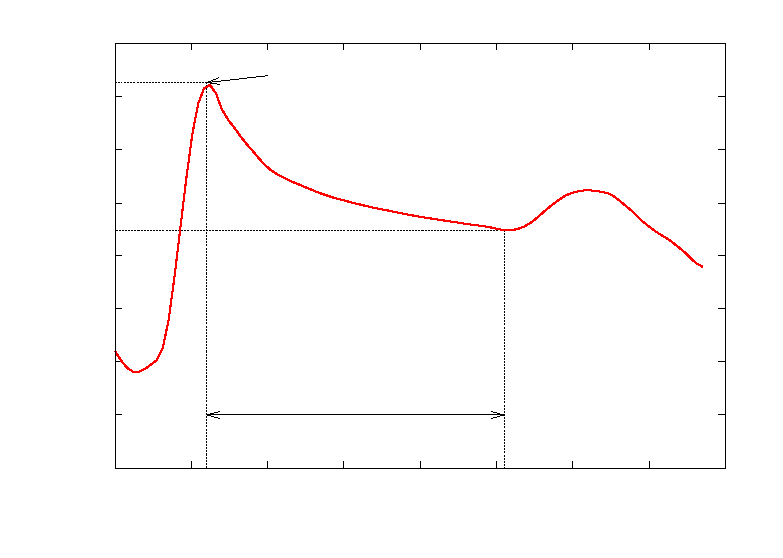
\includegraphics{src/example/hakee}}%
    \gplfronttext
  \end{picture}%
\endgroup

    \end{center}
    \caption{CPVC 转矩-时间 曲线示例图}
    \label{figExHakee}
\end{figure}

\subsection{拉伸性能测试}
拉伸强度定义为断裂前试样所能承受的最大应力,单位为 MPa,用来评价材料的抗拉性能。拉伸强度的计算公式见式 \eqref{eqTenS},其中 $P$ 为样品承受的最大载荷,$b$ 和 $d$ 分别为试样的宽度和厚度。

\begin{equation}
    \label{eqTenS}
    \sigma_t = \frac{P}{bd}
\end{equation}

本实验中采用万能试验机进行拉伸强度测试\footnote{执行标准 GB/T 1040.2-2006},设置拉伸速率为 10 mm/min,夹具距离为 80 mm,样条的最窄宽度为 6 mm,厚度为 4 mm。

\subsection{弯曲性能测试}
弯曲强度是指材料在弯曲负荷作用下破裂或达到规定弯矩时能承受的最大应力,此应力为弯曲时的最大正应力,以 MPa 为单位。它反映了材料抗弯曲的能力,用来评价材料的弯曲性能。横力弯曲时,弯矩 M 随截面位置变化,一般情况下,最大正应力 $\sigma_{max}$ 发生于弯矩最大的截面上,且离中性轴最远处。因此,最大正应力不仅与弯矩 M 有关,还与截面形状和尺寸有关。最大正应力计算公式见式 \eqref{eqBendS},其中 $\sigma_{max}$ 为最大弯矩,$W$ 为抗弯截面系数。

\begin{equation}
    \label{eqBendS}
    \sigma_{max} = \frac{M_{max}}{W}
\end{equation}

本实验同样使用万能试验机进行弯曲强度测试\footnote{执行标准 GB/T 9341-2008},设置移动速率为 2 mm/min,样条尺寸为 80 mm$\times$10 mm$\times$4 mm,跨度为 64 mm。

\subsection{冲击性能测试}
冲击强度是材料在受到冲击后断裂吸收冲击能量的能力,用于评价材料的抗冲击能力或判断材料的脆性和韧性程度。缺口冲击强度的计算公式见式 \eqref{eqImpactS},其中 $aiN$ 为缺口冲击强度(Izod impact strength of a notched specimen),$x\%$ 为实验测得百分比,$S$ 为缺口处截面面积。

\begin{equation}
    \label{eqImpactS}
    aiN = (\frac{2.57 J \times x\%}{S}) KJ/m^2
\end{equation}

本实验采用落锤冲击强度仪进行缺口冲击强度测试\footnote{执行标准 ISO 180/1A},缺口形状为“V”形,深度为 2 mm,落锤满载能量为 2.75 J。

% \subsection{扫描电镜测试}
% SEM 的最大特点是图像富有立体感,放大倍数连续可变,特别适合表面形态的研究,是研究固体材料表面三维结构形态的有效工具,成为常用的高分子表面形貌剖析手段。

\subsection{动态力学热分析(DMA)}
本实验中采用 DMA 对玻璃化转变温度进行测试。DMA 是对试样施加恒定振幅的正弦交变应力,使其发生受迫振动,观察应变随温度或时间的变化规律,从而计算力学参数用以表征材料粘弹性的一种试验方法。在聚合物玻璃化转变过程中,其粘弹性有很大变化,从而可用 DMA 测定 $T_g$。DMA 曲线通常有储能模量、损耗模量、损耗因子这三个信号,对应的 $T_g$ 也可有三种取法,分别为储能模量的台阶式下降曲线部分的起始点、损耗模量的峰值温度、损耗因子\footnote{损耗角正切:$tan \, \delta = \frac{G''}{G'}$}的峰值温度。本实验取损耗因子的峰值温度作为最终测试得到的玻璃化转变温度。如图 \ref{figExTg} 所示,在加热过程中,样品的损耗因子出现了一个峰值,取峰值所在温度为样品的玻璃化转变温度。

\begin{figure}[!htb]
    \begin{center}
        % GNUPLOT: LaTeX picture with Postscript
\begingroup
  \makeatletter
  \providecommand\color[2][]{%
    \GenericError{(gnuplot) \space\space\space\@spaces}{%
      Package color not loaded in conjunction with
      terminal option `colourtext'%
    }{See the gnuplot documentation for explanation.%
    }{Either use 'blacktext' in gnuplot or load the package
      color.sty in LaTeX.}%
    \renewcommand\color[2][]{}%
  }%
  \providecommand\includegraphics[2][]{%
    \GenericError{(gnuplot) \space\space\space\@spaces}{%
      Package graphicx or graphics not loaded%
    }{See the gnuplot documentation for explanation.%
    }{The gnuplot epslatex terminal needs graphicx.sty or graphics.sty.}%
    \renewcommand\includegraphics[2][]{}%
  }%
  \providecommand\rotatebox[2]{#2}%
  \@ifundefined{ifGPcolor}{%
    \newif\ifGPcolor
    \GPcolorfalse
  }{}%
  \@ifundefined{ifGPblacktext}{%
    \newif\ifGPblacktext
    \GPblacktexttrue
  }{}%
  % define a \g@addto@macro without @ in the name:
  \let\gplgaddtomacro\g@addto@macro
  % define empty templates for all commands taking text:
  \gdef\gplbacktext{}%
  \gdef\gplfronttext{}%
  \makeatother
  \ifGPblacktext
    % no textcolor at all
    \def\colorrgb#1{}%
    \def\colorgray#1{}%
  \else
    % gray or color?
    \ifGPcolor
      \def\colorrgb#1{\color[rgb]{#1}}%
      \def\colorgray#1{\color[gray]{#1}}%
      \expandafter\def\csname LTw\endcsname{\color{white}}%
      \expandafter\def\csname LTb\endcsname{\color{black}}%
      \expandafter\def\csname LTa\endcsname{\color{black}}%
      \expandafter\def\csname LT0\endcsname{\color[rgb]{1,0,0}}%
      \expandafter\def\csname LT1\endcsname{\color[rgb]{0,1,0}}%
      \expandafter\def\csname LT2\endcsname{\color[rgb]{0,0,1}}%
      \expandafter\def\csname LT3\endcsname{\color[rgb]{1,0,1}}%
      \expandafter\def\csname LT4\endcsname{\color[rgb]{0,1,1}}%
      \expandafter\def\csname LT5\endcsname{\color[rgb]{1,1,0}}%
      \expandafter\def\csname LT6\endcsname{\color[rgb]{0,0,0}}%
      \expandafter\def\csname LT7\endcsname{\color[rgb]{1,0.3,0}}%
      \expandafter\def\csname LT8\endcsname{\color[rgb]{0.5,0.5,0.5}}%
    \else
      % gray
      \def\colorrgb#1{\color{black}}%
      \def\colorgray#1{\color[gray]{#1}}%
      \expandafter\def\csname LTw\endcsname{\color{white}}%
      \expandafter\def\csname LTb\endcsname{\color{black}}%
      \expandafter\def\csname LTa\endcsname{\color{black}}%
      \expandafter\def\csname LT0\endcsname{\color{black}}%
      \expandafter\def\csname LT1\endcsname{\color{black}}%
      \expandafter\def\csname LT2\endcsname{\color{black}}%
      \expandafter\def\csname LT3\endcsname{\color{black}}%
      \expandafter\def\csname LT4\endcsname{\color{black}}%
      \expandafter\def\csname LT5\endcsname{\color{black}}%
      \expandafter\def\csname LT6\endcsname{\color{black}}%
      \expandafter\def\csname LT7\endcsname{\color{black}}%
      \expandafter\def\csname LT8\endcsname{\color{black}}%
    \fi
  \fi
    \setlength{\unitlength}{0.0500bp}%
    \ifx\gptboxheight\undefined%
      \newlength{\gptboxheight}%
      \newlength{\gptboxwidth}%
      \newsavebox{\gptboxtext}%
    \fi%
    \setlength{\fboxrule}{0.5pt}%
    \setlength{\fboxsep}{1pt}%
\begin{picture}(7200.00,5040.00)%
    \gplgaddtomacro\gplbacktext{%
      \csname LTb\endcsname%
      \put(814,704){\makebox(0,0)[r]{\strut{}$0$}}%
      \put(814,1518){\makebox(0,0)[r]{\strut{}$0.2$}}%
      \put(814,2332){\makebox(0,0)[r]{\strut{}$0.4$}}%
      \put(814,3147){\makebox(0,0)[r]{\strut{}$0.6$}}%
      \put(814,3961){\makebox(0,0)[r]{\strut{}$0.8$}}%
      \put(814,4775){\makebox(0,0)[r]{\strut{}$1$}}%
      \put(946,484){\makebox(0,0){\strut{}$40$}}%
      \put(1678,484){\makebox(0,0){\strut{}$60$}}%
      \put(2410,484){\makebox(0,0){\strut{}$80$}}%
      \put(3142,484){\makebox(0,0){\strut{}$100$}}%
      \put(3875,484){\makebox(0,0){\strut{}$120$}}%
      \put(4607,484){\makebox(0,0){\strut{}$140$}}%
      \put(5339,484){\makebox(0,0){\strut{}$160$}}%
      \put(6071,484){\makebox(0,0){\strut{}$180$}}%
      \put(6803,484){\makebox(0,0){\strut{}$200$}}%
      \put(1078,4266){\makebox(0,0)[l]{\strut{}$tan \, \delta$ maximun}}%
      \put(4988,924){\rotatebox{90}{\makebox(0,0)[l]{\strut{}$T_g$}}}%
    }%
    \gplgaddtomacro\gplfronttext{%
      \csname LTb\endcsname%
      \put(176,2739){\rotatebox{-270}{\makebox(0,0){\strut{}损耗因子}}}%
      \put(3874,154){\makebox(0,0){\strut{}温度/\cd}}%
    }%
    \gplbacktext
    \put(0,0){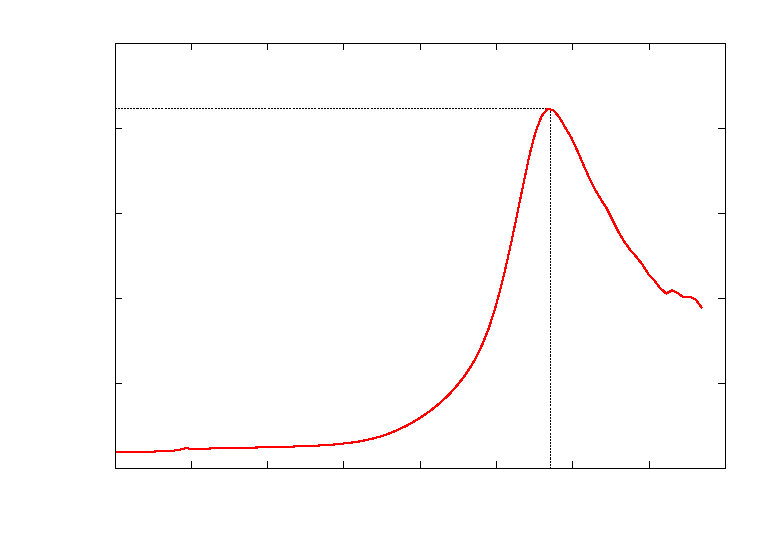
\includegraphics{src/example/tg}}%
    \gplfronttext
  \end{picture}%
\endgroup

    \end{center}
    \caption{CPVC DMA 损耗因子-温度 曲线示例图}
    \label{figExTg}
\end{figure}

\subsection{维卡软化点测试}
维卡软化点是将热塑性塑料置于特定液体传热介质中,在一定的负荷、一定的等速升温条件下,测定试样被 1 $\rm{mm^2}$ 针头压入 1 mm 时的温度\footnote{执行标准 GB 1633-1979}。实验测得的维卡软化点适用于控制质量和作为衡量材料热性能的一个指标,但不代表材料的使用温度。
\chapter{结果与讨论}

\section{润滑体系研究}

\subsection{配方设计}
本实验中使用了 1 种聚乙烯蜡:PEW-0380 以及 3 种氧化聚乙烯蜡:AC-316、AC-617、AC-629。聚乙烯蜡为乙烯的低度聚合产品,具有良好的中期及后期润滑性,并能在 CPVC 注塑加工中作为脱模剂使用。氧化聚乙烯蜡为含羧基的低分子量聚乙烯,并含有醇、酮及酯类化合物。由于氧化使烷烃链上生成一定数量极性的羧基,提高了它在 CPVC 的相容性,使其同时兼有良好的内、外润滑性能,并赋予制品良好的透明性和光泽性。\par
一般认为,外润滑剂的加入会使材料的力学和耐热性能均有所下降。因此我们通过控制其他组成不变,单独改变外润滑剂的种类,从而找到一种在相同用量下能实现最好润滑效果且对材料热稳定性和力学性能影响最小的外润滑剂种类。具体配方如表 \ref{tab1Pre} 所示。

\begin{table}[!htb]
    \caption{CPVC 4 种外润滑剂配方设计表}
    \label{tab1Pre}
    \begin{center}
    \footnotesize{
        \begin{tabular}{ccccccccccc}
            \borderLine
            组别 & CPVC & \makecell[c]{抗冲击\\改性剂} & 有机锡 & \makecell[c]{AC-\\316} & \makecell[c]{AC-\\617} & \makecell[c]{AC-\\629} & \makecell[c]{PEW-\\0380} & \makecell[c]{汉高\\G-60} & \makecell[c]{加工\\助剂} & \makecell[c]{钛白粉}   \\
            \interLine
            $E_1$ & 100 & 8 & 2 & 1.3 & & & & 1.2 & 3 & 2   \\
            $E_2$ & 100 & 8 & 2 & & 1.3 & & & 1.2 & 3 & 2   \\
            $E_3$ & 100 & 8 & 2 & & & 1.3 & & 1.2 & 3 & 2   \\
            $E_4$ & 100 & 8 & 2 & & & & 1.3 & 1.2 & 3 & 2   \\
            \borderLine
        \end{tabular}
    }
    \end{center}
\end{table}

\subsection{热老化试验箱法}

将 4 组配方的样板进行切割,取 1 $\rm{cm^2}$ 的试样进行测试,结果如表 \ref{tab1static} 所示。

\begin{table}[!htb]
    \caption{$E_1 \sim E_4$ 组热老化试验箱法样品颜色随时间变化}
    \label{tab1static}
    \begin{center}
    \footnotesize{
        \begin{tabular}{cccccccc}
            \borderLine
            \multirow{2}{*}{Sample} & \multicolumn{7}{c}{加入不同种类润滑剂的 CPVC 试样 180\cd 烘箱中颜色随时间的变化}\\
            \cline{2-8}
            & 0 min & 20 min & 30 min & 70 min & 120 min & 250 min & 360 min  \\
            \interLine 
            $E_1$ & \makecell[c]{
\includegraphics[width=.1\linewidth]{src/origin/1/static/00.png}} & \makecell[c]{
\includegraphics[width=.1\linewidth]{src/origin/1/static/01.png}} & \makecell[c]{
\includegraphics[width=.1\linewidth]{src/origin/1/static/02.png}} & \makecell[c]{
\includegraphics[width=.1\linewidth]{src/origin/1/static/03.png}} & \makecell[c]{
\includegraphics[width=.1\linewidth]{src/origin/1/static/04.png}} & \makecell[c]{
\includegraphics[width=.1\linewidth]{src/origin/1/static/05.png}} & \makecell[c]{
\includegraphics[width=.1\linewidth]{src/origin/1/static/06.png}}   \\
            $E_2$ & \makecell[c]{
\includegraphics[width=.1\linewidth]{src/origin/1/static/10.png}} & \makecell[c]{
\includegraphics[width=.1\linewidth]{src/origin/1/static/11.png}} & \makecell[c]{
\includegraphics[width=.1\linewidth]{src/origin/1/static/12.png}} & \makecell[c]{
\includegraphics[width=.1\linewidth]{src/origin/1/static/13.png}} & \makecell[c]{
\includegraphics[width=.1\linewidth]{src/origin/1/static/14.png}} & \makecell[c]{
\includegraphics[width=.1\linewidth]{src/origin/1/static/15.png}} & \makecell[c]{
\includegraphics[width=.1\linewidth]{src/origin/1/static/16.png}}  \\
            $E_3$ & \makecell[c]{
\includegraphics[width=.1\linewidth]{src/origin/1/static/20.png}} & \makecell[c]{
\includegraphics[width=.1\linewidth]{src/origin/1/static/21.png}} & \makecell[c]{
\includegraphics[width=.1\linewidth]{src/origin/1/static/22.png}} & \makecell[c]{
\includegraphics[width=.1\linewidth]{src/origin/1/static/23.png}} & \makecell[c]{
\includegraphics[width=.1\linewidth]{src/origin/1/static/24.png}} & \makecell[c]{
\includegraphics[width=.1\linewidth]{src/origin/1/static/25.png}} & \makecell[c]{
\includegraphics[width=.1\linewidth]{src/origin/1/static/26.png}}  \\
            $E_4$ & \makecell[c]{
\includegraphics[width=.1\linewidth]{src/origin/1/static/30.png}} & \makecell[c]{
\includegraphics[width=.1\linewidth]{src/origin/1/static/31.png}} & \makecell[c]{
\includegraphics[width=.1\linewidth]{src/origin/1/static/32.png}} & \makecell[c]{
\includegraphics[width=.1\linewidth]{src/origin/1/static/33.png}} & \makecell[c]{
\includegraphics[width=.1\linewidth]{src/origin/1/static/34.png}} & \makecell[c]{
\includegraphics[width=.1\linewidth]{src/origin/1/static/35.png}} & \makecell[c]{
\includegraphics[width=.1\linewidth]{src/origin/1/static/36.png}}    \\
            \borderLine
        \end{tabular}
    }
    \end{center}
\end{table}

从表 \ref{tab1static} 可以看出,$E_1$ 组和 $E_2$ 组的样品在实验开始的 20 min 后表面开始出现起伏,当 360 min 时,其表面已严重变黑且因 CPVC 分解产生 HCl 而形成了大量的气泡。说明 AC-316 与 AC-617 对 CPVC 树脂的塑化效果改善不大,CPVC 树脂由于塑化不佳致其容易发生分解。$E_4$ 组在 360 min 时轻微发黄,认为 PEW-0380 对 CPVC 塑化效果改善最大。

\subsection{动态热稳定性测试}

图 \ref{fig1Hakee} 所示为 $E_1 \sim E_4$ 四种配方在转矩流变仪中进行加热剪切过程的 转矩-时间 曲线。由图中数据可得到该体系的熔化转矩、平衡转矩与热稳定时间\footnote{见 \pageref{sectionHakee} 页 \ref{sectionHakee} 动态热稳定性},具体数据见表 \ref{tab1Hakee}所示。

\begin{figure}[!htb]
    \begin{center}
        % GNUPLOT: LaTeX picture with Postscript
\begingroup
  \makeatletter
  \providecommand\color[2][]{%
    \GenericError{(gnuplot) \space\space\space\@spaces}{%
      Package color not loaded in conjunction with
      terminal option `colourtext'%
    }{See the gnuplot documentation for explanation.%
    }{Either use 'blacktext' in gnuplot or load the package
      color.sty in LaTeX.}%
    \renewcommand\color[2][]{}%
  }%
  \providecommand\includegraphics[2][]{%
    \GenericError{(gnuplot) \space\space\space\@spaces}{%
      Package graphicx or graphics not loaded%
    }{See the gnuplot documentation for explanation.%
    }{The gnuplot epslatex terminal needs graphicx.sty or graphics.sty.}%
    \renewcommand\includegraphics[2][]{}%
  }%
  \providecommand\rotatebox[2]{#2}%
  \@ifundefined{ifGPcolor}{%
    \newif\ifGPcolor
    \GPcolorfalse
  }{}%
  \@ifundefined{ifGPblacktext}{%
    \newif\ifGPblacktext
    \GPblacktexttrue
  }{}%
  % define a \g@addto@macro without @ in the name:
  \let\gplgaddtomacro\g@addto@macro
  % define empty templates for all commands taking text:
  \gdef\gplbacktext{}%
  \gdef\gplfronttext{}%
  \makeatother
  \ifGPblacktext
    % no textcolor at all
    \def\colorrgb#1{}%
    \def\colorgray#1{}%
  \else
    % gray or color?
    \ifGPcolor
      \def\colorrgb#1{\color[rgb]{#1}}%
      \def\colorgray#1{\color[gray]{#1}}%
      \expandafter\def\csname LTw\endcsname{\color{white}}%
      \expandafter\def\csname LTb\endcsname{\color{black}}%
      \expandafter\def\csname LTa\endcsname{\color{black}}%
      \expandafter\def\csname LT0\endcsname{\color[rgb]{1,0,0}}%
      \expandafter\def\csname LT1\endcsname{\color[rgb]{0,1,0}}%
      \expandafter\def\csname LT2\endcsname{\color[rgb]{0,0,1}}%
      \expandafter\def\csname LT3\endcsname{\color[rgb]{1,0,1}}%
      \expandafter\def\csname LT4\endcsname{\color[rgb]{0,1,1}}%
      \expandafter\def\csname LT5\endcsname{\color[rgb]{1,1,0}}%
      \expandafter\def\csname LT6\endcsname{\color[rgb]{0,0,0}}%
      \expandafter\def\csname LT7\endcsname{\color[rgb]{1,0.3,0}}%
      \expandafter\def\csname LT8\endcsname{\color[rgb]{0.5,0.5,0.5}}%
    \else
      % gray
      \def\colorrgb#1{\color{black}}%
      \def\colorgray#1{\color[gray]{#1}}%
      \expandafter\def\csname LTw\endcsname{\color{white}}%
      \expandafter\def\csname LTb\endcsname{\color{black}}%
      \expandafter\def\csname LTa\endcsname{\color{black}}%
      \expandafter\def\csname LT0\endcsname{\color{black}}%
      \expandafter\def\csname LT1\endcsname{\color{black}}%
      \expandafter\def\csname LT2\endcsname{\color{black}}%
      \expandafter\def\csname LT3\endcsname{\color{black}}%
      \expandafter\def\csname LT4\endcsname{\color{black}}%
      \expandafter\def\csname LT5\endcsname{\color{black}}%
      \expandafter\def\csname LT6\endcsname{\color{black}}%
      \expandafter\def\csname LT7\endcsname{\color{black}}%
      \expandafter\def\csname LT8\endcsname{\color{black}}%
    \fi
  \fi
    \setlength{\unitlength}{0.0500bp}%
    \ifx\gptboxheight\undefined%
      \newlength{\gptboxheight}%
      \newlength{\gptboxwidth}%
      \newsavebox{\gptboxtext}%
    \fi%
    \setlength{\fboxrule}{0.5pt}%
    \setlength{\fboxsep}{1pt}%
\begin{picture}(7200.00,5040.00)%
    \gplgaddtomacro\gplbacktext{%
      \csname LTb\endcsname%
      \put(814,704){\makebox(0,0)[r]{\strut{}$-10$}}%
      \put(814,1213){\makebox(0,0)[r]{\strut{}$-5$}}%
      \put(814,1722){\makebox(0,0)[r]{\strut{}$0$}}%
      \put(814,2231){\makebox(0,0)[r]{\strut{}$5$}}%
      \put(814,2740){\makebox(0,0)[r]{\strut{}$10$}}%
      \put(814,3248){\makebox(0,0)[r]{\strut{}$15$}}%
      \put(814,3757){\makebox(0,0)[r]{\strut{}$20$}}%
      \put(814,4266){\makebox(0,0)[r]{\strut{}$25$}}%
      \put(814,4775){\makebox(0,0)[r]{\strut{}$30$}}%
      \put(946,484){\makebox(0,0){\strut{}$0$}}%
      \put(1678,484){\makebox(0,0){\strut{}$1$}}%
      \put(2410,484){\makebox(0,0){\strut{}$2$}}%
      \put(3142,484){\makebox(0,0){\strut{}$3$}}%
      \put(3875,484){\makebox(0,0){\strut{}$4$}}%
      \put(4607,484){\makebox(0,0){\strut{}$5$}}%
      \put(5339,484){\makebox(0,0){\strut{}$6$}}%
      \put(6071,484){\makebox(0,0){\strut{}$7$}}%
      \put(6803,484){\makebox(0,0){\strut{}$8$}}%
    }%
    \gplgaddtomacro\gplfronttext{%
      \csname LTb\endcsname%
      \put(176,2739){\rotatebox{-270}{\makebox(0,0){\strut{}转矩/N$\cdot$m}}}%
      \put(3874,154){\makebox(0,0){\strut{}时间/min}}%
      \csname LTb\endcsname%
      \put(5816,1537){\makebox(0,0)[r]{\strut{}AC-316}}%
      \csname LTb\endcsname%
      \put(5816,1317){\makebox(0,0)[r]{\strut{}AC-617}}%
      \csname LTb\endcsname%
      \put(5816,1097){\makebox(0,0)[r]{\strut{}AC-629}}%
      \csname LTb\endcsname%
      \put(5816,877){\makebox(0,0)[r]{\strut{}PEW-0380}}%
    }%
    \gplbacktext
    \put(0,0){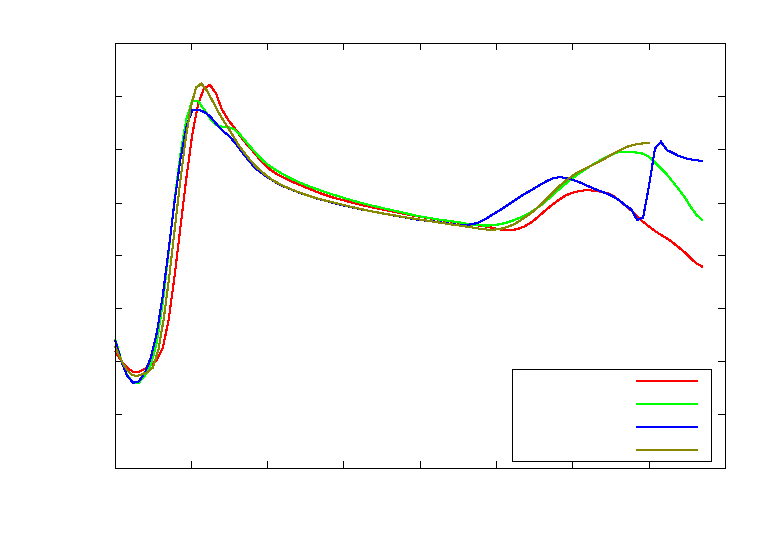
\includegraphics{src/origin/1/hakee}}%
    \gplfronttext
  \end{picture}%
\endgroup

    \end{center}
    \caption{$E_1 \sim E_4$ 组转矩流变仪 转矩-时间 曲线}
    \label{fig1Hakee}
\end{figure}

\begin{table}[!htb]
    \caption{$E_1 \sim E_4$ 组动态热稳定性能数据表}
    \label{tab1Hakee}
    \begin{center}
    \footnotesize{
        \begin{tabular}{ccccc}
            \borderLine
            组别 & 润滑剂种类 & \makecell[c]{熔化转矩 $M_{fus}$/\\N$\cdot$m} & \makecell[c]{平衡转矩$M_{melt}$/\\N$\cdot$m} & \makecell[c]{热稳定时间$T_{s}$/\\min} \\
            \interLine
            $E_1$ & AC-316 & 29.6 & 12.1 & 6.2  \\
            $E_2$ & AC-617 & 26.5 & 12.5 & 6.6  \\
            $E_3$ & AC-629 & 24.9 & 12.4 & 5.9  \\
            $E_4$ & PEW-0380 & 28.0 & 12.2 & 7.3    \\
            \borderLine
        \end{tabular}
    }
    \end{center}
\end{table}

结合图表数据可以看出,将试样加入到转矩流变仪后,$E_2$ 组和 $E_3$ 组的熔化转矩明显小于 $E_1$ 组和 $E_4$ 组,认为 $E_2$ 组和 $E_3$ 组的混合物熔体黏度小于 $E_1$ 组和 $E_4$ 组。考虑到 4 种外润滑剂的黏度相差较大,分析是 AC-316 和 PEW-0380 的黏度较 AC-617 和 AC-629 的大,因此在熔化初期其在 CPVC 熔体表面的分布不佳,导致熔化转矩相对较高。随着时间的进行,$E_2$ 组和 $E_3$ 组首先到达平衡转矩的最低点,并且该其平衡转矩略大于 $E_1$ 组和 $E_4$ 组,因此认为在长时间的塑化过程中,AC-316 与 PEW-0380 仍能保持较好的润滑效果,原因为 AC-617 与 AC-629 的滴点较 AC-316 与 PEW-0380 更低,因此在塑化加工过程中,温度逐渐上升,AC-617 与 AC-629 首先失效 导致其平衡转矩较大,加工性能变差。$E_4$ 组具有最长的热稳定时间,其 $T_{s}$ 为 7.3 min,能够满足 CPVC 塑化加工的要求。

\subsection{力学性能测试}

采用万能试验机对 $E_1 \sim E_4$ 组的标准试样进行拉伸强度、弯曲强度和缺口冲击强度的测试,具体数据如表 \ref{tab1Mach} 所示。

\begin{table}[!htb]
    \caption{$E_1 \sim E_4$ 组力学性能数据表}
    \label{tab1Mach}
    \begin{center}
    \footnotesize{
        \begin{tabular}{cccc}
			\borderLine
			组别 & \makecell[c]{拉伸强度$\sigma_t$/\\MPa} & \makecell[c]{弯曲强度$\sigma_{b}$/\\Mpa} & \makecell[c]{缺口冲击强度$aiN$/\\$\rm{KJ/m^2}$}\\
			\interLine
			$E_1$ & 57.30 & 63.73 & 8.01	\\
			$E_2$ & 59.16 & 60.29 & 10.57	\\
			$E_3$ & 58.77 & 60.59 & 14.10	\\
			$E_4$ & 59.48 & 60.61 & 16.04	\\
			\borderLine
        \end{tabular}
    }
    \end{center}
\end{table}

从表中数据可见,四组的拉伸强度和弯曲强度差别不大,但缺口冲击强度呈 $aiN_{E_4} > aiN_{E_3} > aiN_{E_2} > aiN_{E_1}$ 的趋势,并且 $E_4$ 组的缺口冲击强度远好于 $E_1$ 组 和 $E_2$ 组。分析原因为 PEW-0380 在 CPVC 的塑化过程中,能够保持较好的润滑作用,使得 CPVC 分子在较少发生热分解的情况下部分断裂生成分子量较小的 CPVC 链,从而实现较好的塑化效果。这部分较短的 CPVC 分子链为体系提供了很大的冲击强度以及韧性的改善。

\subsection{动态力学热分析(DMA)}

根据 $E_1 \sim E_4$ 四组配方的 损耗因子-时间 数据制得图 \ref{fig1Tg},取损耗因子的峰值温度作为试样的玻璃化转变温度。

\begin{figure}[!htb]
    \begin{center}
        % GNUPLOT: LaTeX picture with Postscript
\begingroup
  \makeatletter
  \providecommand\color[2][]{%
    \GenericError{(gnuplot) \space\space\space\@spaces}{%
      Package color not loaded in conjunction with
      terminal option `colourtext'%
    }{See the gnuplot documentation for explanation.%
    }{Either use 'blacktext' in gnuplot or load the package
      color.sty in LaTeX.}%
    \renewcommand\color[2][]{}%
  }%
  \providecommand\includegraphics[2][]{%
    \GenericError{(gnuplot) \space\space\space\@spaces}{%
      Package graphicx or graphics not loaded%
    }{See the gnuplot documentation for explanation.%
    }{The gnuplot epslatex terminal needs graphicx.sty or graphics.sty.}%
    \renewcommand\includegraphics[2][]{}%
  }%
  \providecommand\rotatebox[2]{#2}%
  \@ifundefined{ifGPcolor}{%
    \newif\ifGPcolor
    \GPcolorfalse
  }{}%
  \@ifundefined{ifGPblacktext}{%
    \newif\ifGPblacktext
    \GPblacktexttrue
  }{}%
  % define a \g@addto@macro without @ in the name:
  \let\gplgaddtomacro\g@addto@macro
  % define empty templates for all commands taking text:
  \gdef\gplbacktext{}%
  \gdef\gplfronttext{}%
  \makeatother
  \ifGPblacktext
    % no textcolor at all
    \def\colorrgb#1{}%
    \def\colorgray#1{}%
  \else
    % gray or color?
    \ifGPcolor
      \def\colorrgb#1{\color[rgb]{#1}}%
      \def\colorgray#1{\color[gray]{#1}}%
      \expandafter\def\csname LTw\endcsname{\color{white}}%
      \expandafter\def\csname LTb\endcsname{\color{black}}%
      \expandafter\def\csname LTa\endcsname{\color{black}}%
      \expandafter\def\csname LT0\endcsname{\color[rgb]{1,0,0}}%
      \expandafter\def\csname LT1\endcsname{\color[rgb]{0,1,0}}%
      \expandafter\def\csname LT2\endcsname{\color[rgb]{0,0,1}}%
      \expandafter\def\csname LT3\endcsname{\color[rgb]{1,0,1}}%
      \expandafter\def\csname LT4\endcsname{\color[rgb]{0,1,1}}%
      \expandafter\def\csname LT5\endcsname{\color[rgb]{1,1,0}}%
      \expandafter\def\csname LT6\endcsname{\color[rgb]{0,0,0}}%
      \expandafter\def\csname LT7\endcsname{\color[rgb]{1,0.3,0}}%
      \expandafter\def\csname LT8\endcsname{\color[rgb]{0.5,0.5,0.5}}%
    \else
      % gray
      \def\colorrgb#1{\color{black}}%
      \def\colorgray#1{\color[gray]{#1}}%
      \expandafter\def\csname LTw\endcsname{\color{white}}%
      \expandafter\def\csname LTb\endcsname{\color{black}}%
      \expandafter\def\csname LTa\endcsname{\color{black}}%
      \expandafter\def\csname LT0\endcsname{\color{black}}%
      \expandafter\def\csname LT1\endcsname{\color{black}}%
      \expandafter\def\csname LT2\endcsname{\color{black}}%
      \expandafter\def\csname LT3\endcsname{\color{black}}%
      \expandafter\def\csname LT4\endcsname{\color{black}}%
      \expandafter\def\csname LT5\endcsname{\color{black}}%
      \expandafter\def\csname LT6\endcsname{\color{black}}%
      \expandafter\def\csname LT7\endcsname{\color{black}}%
      \expandafter\def\csname LT8\endcsname{\color{black}}%
    \fi
  \fi
    \setlength{\unitlength}{0.0500bp}%
    \ifx\gptboxheight\undefined%
      \newlength{\gptboxheight}%
      \newlength{\gptboxwidth}%
      \newsavebox{\gptboxtext}%
    \fi%
    \setlength{\fboxrule}{0.5pt}%
    \setlength{\fboxsep}{1pt}%
\begin{picture}(7200.00,5040.00)%
    \gplgaddtomacro\gplbacktext{%
      \csname LTb\endcsname%
      \put(814,704){\makebox(0,0)[r]{\strut{}$0$}}%
      \put(814,1518){\makebox(0,0)[r]{\strut{}$0.2$}}%
      \put(814,2332){\makebox(0,0)[r]{\strut{}$0.4$}}%
      \put(814,3147){\makebox(0,0)[r]{\strut{}$0.6$}}%
      \put(814,3961){\makebox(0,0)[r]{\strut{}$0.8$}}%
      \put(814,4775){\makebox(0,0)[r]{\strut{}$1$}}%
      \put(946,484){\makebox(0,0){\strut{}$40$}}%
      \put(1678,484){\makebox(0,0){\strut{}$60$}}%
      \put(2410,484){\makebox(0,0){\strut{}$80$}}%
      \put(3142,484){\makebox(0,0){\strut{}$100$}}%
      \put(3875,484){\makebox(0,0){\strut{}$120$}}%
      \put(4607,484){\makebox(0,0){\strut{}$140$}}%
      \put(5339,484){\makebox(0,0){\strut{}$160$}}%
      \put(6071,484){\makebox(0,0){\strut{}$180$}}%
      \put(6803,484){\makebox(0,0){\strut{}$200$}}%
    }%
    \gplgaddtomacro\gplfronttext{%
      \csname LTb\endcsname%
      \put(176,2739){\rotatebox{-270}{\makebox(0,0){\strut{}损耗角正切}}}%
      \put(3874,154){\makebox(0,0){\strut{}温度/\cd}}%
      \csname LTb\endcsname%
      \put(2134,4602){\makebox(0,0)[r]{\strut{}AC-316}}%
      \csname LTb\endcsname%
      \put(2134,4382){\makebox(0,0)[r]{\strut{}AC-617}}%
      \csname LTb\endcsname%
      \put(2134,4162){\makebox(0,0)[r]{\strut{}AC-629}}%
      \csname LTb\endcsname%
      \put(2134,3942){\makebox(0,0)[r]{\strut{}PEW-0380}}%
    }%
    \gplbacktext
    \put(0,0){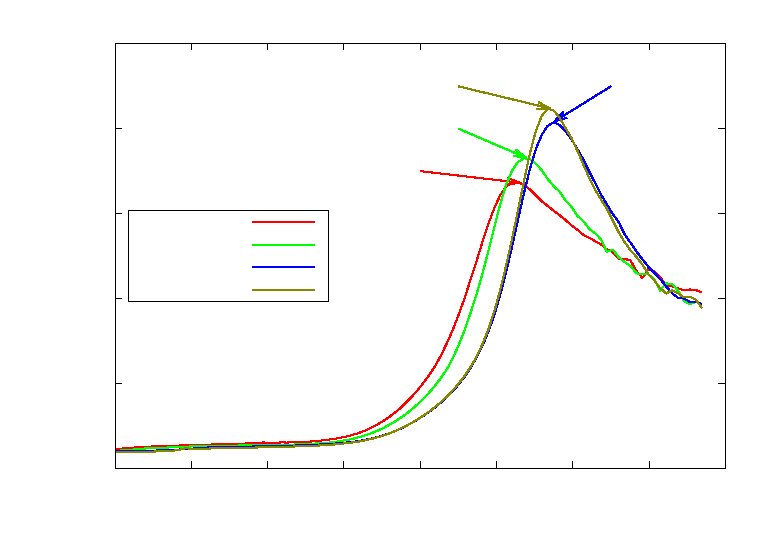
\includegraphics{src/origin/1/tg}}%
    \gplfronttext
  \end{picture}%
\endgroup

    \end{center}
    \caption{外润滑剂玻璃化转变温度}
    \label{fig1Tg}
\end{figure}

根据实验结果,$E_3$ 和 $E_4$ 组具有较高的玻璃化温度,分别为 155.17\cd 和 154.03\cd,比 $E_1$ 和 $E_2$ 组的 146.09\cd 和 147.78\cd 平均高 7\cd 左右。本实验结果与静态热稳定性测试的结果一致,认为玻璃化温度、静态热稳定性与 CPVC 的塑化效果呈正相关。在塑化过程中 AC-316 与 AC-617 对 CPVC 的塑化效果较差,导致体系的受热均匀性也较差。CPVC 分子易发生断裂,或分解脱除 HCl,最终形成分子量较小同时双键较多的分子链。最终 $E_1$ 和 $E_2$ 组的 $T_g$ 较低。

\subsection{本节小结}
本节实验对 AC-316、AC-617、AC-629 和 PEW-0380 四种外润滑剂进行了热性能和力学性能的测试。结果表明,AC-629 与 PEW-0380 外润滑剂为 CPVC 提供较好的润滑效果和塑化效果,使其热稳定性也略好于 AC-316 和 AC-617 组。但由于 AC-617、AC-629 的滴点较低,使其在加工过程中较早失效,使得加工能耗上升。在力学性能的测试中,4 组试样具有相近的拉伸强度与弯曲强度,但 PEW-0380 能使 CPVC 提供最好的冲击强度。因此在加工过程中,若加工温度不高,则外润滑剂可选用润滑效果较好的 AC-629 与 PEW-0380,若加工温度较高,则选用滴点较高的 AC-316 与 PEW-0380。


\section{热稳定体系研究}

\subsection{配方设计}
在本组实验中,我们使用了 TMG-234、T-190A 以及祥生公司的液体有机锡进行测试。有机锡稳定剂的稳定效果较好,可通过特殊的配位作用取代 CPVC 分子上的烯丙基氯原子。但有机锡稳定剂的价格较高,因此我们希望寻找一种在相同用量下稳定效果最好的热稳定剂。因此我们通过控制其他组成不变,单独改变有机锡稳定剂的种类,从而找到一种在相同用量下能实现最好稳定效果且对材料力学性能影响最小的有机锡热稳定剂。具体配方如表 \ref{tab3Pre} 所示。

\begin{table}[!htb]
    \caption{CPVC 3 种有机锡热稳定剂配方设计表}
    \label{tab3Pre}
    \begin{center}
    \footnotesize{
        \begin{tabular}{cccccccccc}
            \borderLine
			组别 & CPVC & \makecell[c]{抗冲击\\改性剂} & \makecell[c]{TMG-\\234} & \makecell[c]{T-\\190A} & \makecell[c]{液体\\有机锡} & 外润滑剂 & 内润滑剂 & 加工助剂 & 钛白粉	\\
            \interLine
            $T_1$ & 100 & 8 & 2 & & & 1.3 & 1.2 & 3 & 2	\\
            $T_2$ & 100 & 8 & & 2 & & 1.3 & 1.2 & 3 & 2	\\
            $T_3$ & 100 & 8 & & & 2 & 1.3 & 1.2 & 3 & 2	\\
            \borderLine
        \end{tabular}
    }
    \end{center}
\end{table}

\subsection{热老化试验箱法}
将 3 组配方的样板进行切割,取 1 $\rm{cm^2}$ 的试样进行测试,结果如表 \ref{tab3static} 所示。

\begin{table}[!htb]
    \caption{$T_1 \sim T_3$ 组热老化试验箱法样品颜色随时间变化}
    \label{tab3static}
    \begin{center}
    \footnotesize{
        \begin{tabular}{cccccccc}
            \borderLine
            \multirow{2}{*}{Sample} & \multicolumn{7}{c}{加入不同种类稳定剂的 CPVC 试样 180\cd 烘箱中颜色随时间的变化}\\
            \cline{2-8}
            & 0 min & 20 min & 30 min & 70 min & 120 min & 250 min & 360 min  \\
            \interLine 
            $T_1$ & \makecell[c]{
\includegraphics[width=.1\linewidth]{src/origin/3/static/00.png}} & \makecell[c]{
\includegraphics[width=.1\linewidth]{src/origin/3/static/01.png}} & \makecell[c]{
\includegraphics[width=.1\linewidth]{src/origin/3/static/02.png}} & \makecell[c]{
\includegraphics[width=.1\linewidth]{src/origin/3/static/03.png}} & \makecell[c]{
\includegraphics[width=.1\linewidth]{src/origin/3/static/04.png}} & \makecell[c]{
\includegraphics[width=.1\linewidth]{src/origin/3/static/05.png}} & \makecell[c]{
\includegraphics[width=.1\linewidth]{src/origin/3/static/06.png}}   \\
            $T_2$ & \makecell[c]{
\includegraphics[width=.1\linewidth]{src/origin/3/static/10.png}} & \makecell[c]{
\includegraphics[width=.1\linewidth]{src/origin/3/static/11.png}} & \makecell[c]{
\includegraphics[width=.1\linewidth]{src/origin/3/static/12.png}} & \makecell[c]{
\includegraphics[width=.1\linewidth]{src/origin/3/static/13.png}} & \makecell[c]{
\includegraphics[width=.1\linewidth]{src/origin/3/static/14.png}} & \makecell[c]{
\includegraphics[width=.1\linewidth]{src/origin/3/static/15.png}} & \makecell[c]{
\includegraphics[width=.1\linewidth]{src/origin/3/static/16.png}}  \\
            $T_3$ & \makecell[c]{
\includegraphics[width=.1\linewidth]{src/origin/3/static/20.png}} & \makecell[c]{
\includegraphics[width=.1\linewidth]{src/origin/3/static/21.png}} & \makecell[c]{
\includegraphics[width=.1\linewidth]{src/origin/3/static/22.png}} & \makecell[c]{
\includegraphics[width=.1\linewidth]{src/origin/3/static/23.png}} & \makecell[c]{\includegraphics[width=.1\linewidth]{src/origin/3/static/24.png}} & \makecell[c]{\includegraphics[width=.1\linewidth]{src/origin/3/static/25.png}} & \makecell[c]{\includegraphics[width=.1\linewidth]{src/origin/3/static/26.png}}  \\
            \borderLine
        \end{tabular}
    }
    \end{center}
\end{table}

从表 \ref{tab3static} 可以看出,$T_1$ 和 $T_2$ 组在静态热稳定性上相近,其在 120 min 之前只是轻微变色,在 360 min 时,$T_1$ 和 $T_2$ 组试样明显变黑但未出现明显气泡,此时 CPVC 发生部分分解,分子中产生双键从而发生氧化变黑,但产生的 HCl 量不足以使试样表面产生气泡,可认为加入 TMG-234 和 T-190A 有机锡的试样热稳定性较好,并且可在 190\cd 下维持较长时间的稳定作用。$T_3$ 组在 120 min 前未出现明显变色,甚至略好于 $T_1$ 和 $T_2$ 组的试样,但从 250 min 分钟开始试样表面出现大量气泡,360 min 时试样严重变黑且表面出现大量瘤状气泡。在较短时间内,液体有机锡与 TMG-234、T-190A 的热稳定效果相近,甚至略好。而在较长时间范围内,TMG-234 和 T-190A 的效果明显优于液体有机锡。本实验也从侧面验证了 CPVC 脱 HCl 的链锁分解机理,当 CPVC 分解产生少量 HCl 后,HCl 的分解量会呈几何增长。

\subsection{动态热稳定性测试}
图 \ref{fig3Hakee} 所示为 $T_1 \sim T_3$ 四种配方在转矩流变仪中进行加热剪切过程的 转矩-时间 曲线。由图中数据可得到该体系的熔化转矩、平衡转矩与热稳定时间,具体数据见表 \ref{tab3Hakee}所示。

\begin{figure}[!htb]
    \begin{center}
        % GNUPLOT: LaTeX picture with Postscript
\begingroup
  \makeatletter
  \providecommand\color[2][]{%
    \GenericError{(gnuplot) \space\space\space\@spaces}{%
      Package color not loaded in conjunction with
      terminal option `colourtext'%
    }{See the gnuplot documentation for explanation.%
    }{Either use 'blacktext' in gnuplot or load the package
      color.sty in LaTeX.}%
    \renewcommand\color[2][]{}%
  }%
  \providecommand\includegraphics[2][]{%
    \GenericError{(gnuplot) \space\space\space\@spaces}{%
      Package graphicx or graphics not loaded%
    }{See the gnuplot documentation for explanation.%
    }{The gnuplot epslatex terminal needs graphicx.sty or graphics.sty.}%
    \renewcommand\includegraphics[2][]{}%
  }%
  \providecommand\rotatebox[2]{#2}%
  \@ifundefined{ifGPcolor}{%
    \newif\ifGPcolor
    \GPcolorfalse
  }{}%
  \@ifundefined{ifGPblacktext}{%
    \newif\ifGPblacktext
    \GPblacktexttrue
  }{}%
  % define a \g@addto@macro without @ in the name:
  \let\gplgaddtomacro\g@addto@macro
  % define empty templates for all commands taking text:
  \gdef\gplbacktext{}%
  \gdef\gplfronttext{}%
  \makeatother
  \ifGPblacktext
    % no textcolor at all
    \def\colorrgb#1{}%
    \def\colorgray#1{}%
  \else
    % gray or color?
    \ifGPcolor
      \def\colorrgb#1{\color[rgb]{#1}}%
      \def\colorgray#1{\color[gray]{#1}}%
      \expandafter\def\csname LTw\endcsname{\color{white}}%
      \expandafter\def\csname LTb\endcsname{\color{black}}%
      \expandafter\def\csname LTa\endcsname{\color{black}}%
      \expandafter\def\csname LT0\endcsname{\color[rgb]{1,0,0}}%
      \expandafter\def\csname LT1\endcsname{\color[rgb]{0,1,0}}%
      \expandafter\def\csname LT2\endcsname{\color[rgb]{0,0,1}}%
      \expandafter\def\csname LT3\endcsname{\color[rgb]{1,0,1}}%
      \expandafter\def\csname LT4\endcsname{\color[rgb]{0,1,1}}%
      \expandafter\def\csname LT5\endcsname{\color[rgb]{1,1,0}}%
      \expandafter\def\csname LT6\endcsname{\color[rgb]{0,0,0}}%
      \expandafter\def\csname LT7\endcsname{\color[rgb]{1,0.3,0}}%
      \expandafter\def\csname LT8\endcsname{\color[rgb]{0.5,0.5,0.5}}%
    \else
      % gray
      \def\colorrgb#1{\color{black}}%
      \def\colorgray#1{\color[gray]{#1}}%
      \expandafter\def\csname LTw\endcsname{\color{white}}%
      \expandafter\def\csname LTb\endcsname{\color{black}}%
      \expandafter\def\csname LTa\endcsname{\color{black}}%
      \expandafter\def\csname LT0\endcsname{\color{black}}%
      \expandafter\def\csname LT1\endcsname{\color{black}}%
      \expandafter\def\csname LT2\endcsname{\color{black}}%
      \expandafter\def\csname LT3\endcsname{\color{black}}%
      \expandafter\def\csname LT4\endcsname{\color{black}}%
      \expandafter\def\csname LT5\endcsname{\color{black}}%
      \expandafter\def\csname LT6\endcsname{\color{black}}%
      \expandafter\def\csname LT7\endcsname{\color{black}}%
      \expandafter\def\csname LT8\endcsname{\color{black}}%
    \fi
  \fi
    \setlength{\unitlength}{0.0500bp}%
    \ifx\gptboxheight\undefined%
      \newlength{\gptboxheight}%
      \newlength{\gptboxwidth}%
      \newsavebox{\gptboxtext}%
    \fi%
    \setlength{\fboxrule}{0.5pt}%
    \setlength{\fboxsep}{1pt}%
\begin{picture}(7200.00,5040.00)%
    \gplgaddtomacro\gplbacktext{%
      \csname LTb\endcsname%
      \put(682,704){\makebox(0,0)[r]{\strut{}$0$}}%
      \put(682,1722){\makebox(0,0)[r]{\strut{}$5$}}%
      \put(682,2740){\makebox(0,0)[r]{\strut{}$10$}}%
      \put(682,3757){\makebox(0,0)[r]{\strut{}$15$}}%
      \put(682,4775){\makebox(0,0)[r]{\strut{}$20$}}%
      \put(814,484){\makebox(0,0){\strut{}$0$}}%
      \put(1903,484){\makebox(0,0){\strut{}$2$}}%
      \put(2992,484){\makebox(0,0){\strut{}$4$}}%
      \put(4081,484){\makebox(0,0){\strut{}$6$}}%
      \put(5170,484){\makebox(0,0){\strut{}$8$}}%
      \put(6259,484){\makebox(0,0){\strut{}$10$}}%
    }%
    \gplgaddtomacro\gplfronttext{%
      \csname LTb\endcsname%
      \put(176,2739){\rotatebox{-270}{\makebox(0,0){\strut{}转矩/N$\cdot$m}}}%
      \put(3808,154){\makebox(0,0){\strut{}时间/min}}%
      \csname LTb\endcsname%
      \put(5816,1317){\makebox(0,0)[r]{\strut{}TMG-234}}%
      \csname LTb\endcsname%
      \put(5816,1097){\makebox(0,0)[r]{\strut{}T-190 A}}%
      \csname LTb\endcsname%
      \put(5816,877){\makebox(0,0)[r]{\strut{}Orgin Tin(l)}}%
    }%
    \gplbacktext
    \put(0,0){\includegraphics{src/origin/3/hakee}}%
    \gplfronttext
  \end{picture}%
\endgroup

    \end{center}
    \caption{$T_1 \sim T_3$ 组转矩流变仪 转矩-时间 曲线}
	\label{fig3Hakee}
\end{figure}

\begin{table}[!htb]
    \caption{$T_1 \sim T_3$ 组动态热稳定性能数据表}
    \label{tab3Hakee}
    \begin{center}
    \footnotesize{
        \begin{tabular}{ccccc}
            \borderLine
            组别 & 热稳定剂 & \makecell[c]{熔化转矩 $M_{fus}$/\\N$\cdot$m} & \makecell[c]{平衡转矩$M_{melt}$/\\N$\cdot$m} & \makecell[c]{热稳定时间$T_{s}$/\\min} \\
            \interLine
            $T_1$ & TMG-234 & 19.8 & 10.8 & 6.5	\\
            $T_2$ & T-190A & 19.1 & 10.3 & 6.1	\\
            $T_3$ & 液体有机锡 & 18.8 & 10.1 & 5.4  \\
            \borderLine
        \end{tabular}
    }
    \end{center}
\end{table}

结合图表数据,我们可以看出 $T_1$ 组的熔化转矩略大于 $T_2$ 组和 $T_3$ 组,同时三组的平衡转矩呈 $M_{melt, T_1} > M_{melt, T_2} > M_{melt, T_3}$ 的趋势,三组的热稳定时间也呈 $T_{s, T_1} > T_{s, T_2} > T_{s, T_3}$ 趋势排列。该组的 平衡转矩与热稳定时间呈较好的正相关性,猜测是在 CPVC 发生大量分解之前,液体有机锡的稳定效果较 TMG-234 和 T-190A 略好,但其长期热稳定性较差,导致体系提前进入热分解阶段。

\subsection{力学性能测试}
采用万能试验机对 $T_1 \sim T_3$ 组的标准试样进行拉伸强度、弯曲强度和缺口冲击强度的测试,具体数据如表 \ref{tab3Mach} 所示。

\begin{table}[!htb]
    \caption{$T_1 \sim T_3$ 组力学性能数据表}
    \label{tab3Mach}
    \begin{center}
    \footnotesize{
        \begin{tabular}{ccccc}
			\borderLine
			组别 & \makecell[c]{拉伸强度$\sigma_t$/\\MPa} & \makecell[c]{弯曲强度$\sigma_{b}$/\\Mpa} & \makecell[c]{缺口冲击强度$aiN$/\\$\rm{KJ/m^2}$} & \makecell[c]{断裂伸长率\\\%}	\\
			\interLine
			$T_1$ & 48.84 & 57.40 & 3.50 & 50.45	\\
			$T_2$ & 53.66 & 61.22 & 5.22 & 62.36	\\
			$T_3$ & 54.10 & 59.21 & 7.95 & 81.36	\\
			\borderLine
        \end{tabular}
    }
    \end{center}
\end{table}

由表 \ref{tab3Mach} 中数据,发现对于拉伸强度、缺口冲击强度、断裂伸长率同样呈现了非常好的正相关性,$T_3$ 组的力学性能参数明显优于 $T_1$ 组和 $T_2$ 组。可以推测,我们在实际的 CPVC 塑化以及压片过程中,塑化时间并未达到液体有机锡的热稳定时间上限,此时液体有机锡的热稳定效果是优于 TMG-234 和 T-190A 的,其在不影响 CPVC 树脂热稳定性的情况下还能提供较好的塑化效果,使得 $T_3$ 组的拉伸强度、缺口冲击强度和断裂伸长率的损失较小。

\subsection{动态力学热分析(DMA)}
根据 $T_1 \sim T_3$ 三组配方的 损耗因子-时间 数据制得图 \ref{fig3Tg},取损耗因子的峰值温度作为试样的玻璃化转变温度。

\begin{figure}[!htb]
    \begin{center}
        % GNUPLOT: LaTeX picture with Postscript
\begingroup
  \makeatletter
  \providecommand\color[2][]{%
    \GenericError{(gnuplot) \space\space\space\@spaces}{%
      Package color not loaded in conjunction with
      terminal option `colourtext'%
    }{See the gnuplot documentation for explanation.%
    }{Either use 'blacktext' in gnuplot or load the package
      color.sty in LaTeX.}%
    \renewcommand\color[2][]{}%
  }%
  \providecommand\includegraphics[2][]{%
    \GenericError{(gnuplot) \space\space\space\@spaces}{%
      Package graphicx or graphics not loaded%
    }{See the gnuplot documentation for explanation.%
    }{The gnuplot epslatex terminal needs graphicx.sty or graphics.sty.}%
    \renewcommand\includegraphics[2][]{}%
  }%
  \providecommand\rotatebox[2]{#2}%
  \@ifundefined{ifGPcolor}{%
    \newif\ifGPcolor
    \GPcolorfalse
  }{}%
  \@ifundefined{ifGPblacktext}{%
    \newif\ifGPblacktext
    \GPblacktexttrue
  }{}%
  % define a \g@addto@macro without @ in the name:
  \let\gplgaddtomacro\g@addto@macro
  % define empty templates for all commands taking text:
  \gdef\gplbacktext{}%
  \gdef\gplfronttext{}%
  \makeatother
  \ifGPblacktext
    % no textcolor at all
    \def\colorrgb#1{}%
    \def\colorgray#1{}%
  \else
    % gray or color?
    \ifGPcolor
      \def\colorrgb#1{\color[rgb]{#1}}%
      \def\colorgray#1{\color[gray]{#1}}%
      \expandafter\def\csname LTw\endcsname{\color{white}}%
      \expandafter\def\csname LTb\endcsname{\color{black}}%
      \expandafter\def\csname LTa\endcsname{\color{black}}%
      \expandafter\def\csname LT0\endcsname{\color[rgb]{1,0,0}}%
      \expandafter\def\csname LT1\endcsname{\color[rgb]{0,1,0}}%
      \expandafter\def\csname LT2\endcsname{\color[rgb]{0,0,1}}%
      \expandafter\def\csname LT3\endcsname{\color[rgb]{1,0,1}}%
      \expandafter\def\csname LT4\endcsname{\color[rgb]{0,1,1}}%
      \expandafter\def\csname LT5\endcsname{\color[rgb]{1,1,0}}%
      \expandafter\def\csname LT6\endcsname{\color[rgb]{0,0,0}}%
      \expandafter\def\csname LT7\endcsname{\color[rgb]{1,0.3,0}}%
      \expandafter\def\csname LT8\endcsname{\color[rgb]{0.5,0.5,0.5}}%
    \else
      % gray
      \def\colorrgb#1{\color{black}}%
      \def\colorgray#1{\color[gray]{#1}}%
      \expandafter\def\csname LTw\endcsname{\color{white}}%
      \expandafter\def\csname LTb\endcsname{\color{black}}%
      \expandafter\def\csname LTa\endcsname{\color{black}}%
      \expandafter\def\csname LT0\endcsname{\color{black}}%
      \expandafter\def\csname LT1\endcsname{\color{black}}%
      \expandafter\def\csname LT2\endcsname{\color{black}}%
      \expandafter\def\csname LT3\endcsname{\color{black}}%
      \expandafter\def\csname LT4\endcsname{\color{black}}%
      \expandafter\def\csname LT5\endcsname{\color{black}}%
      \expandafter\def\csname LT6\endcsname{\color{black}}%
      \expandafter\def\csname LT7\endcsname{\color{black}}%
      \expandafter\def\csname LT8\endcsname{\color{black}}%
    \fi
  \fi
    \setlength{\unitlength}{0.0500bp}%
    \ifx\gptboxheight\undefined%
      \newlength{\gptboxheight}%
      \newlength{\gptboxwidth}%
      \newsavebox{\gptboxtext}%
    \fi%
    \setlength{\fboxrule}{0.5pt}%
    \setlength{\fboxsep}{1pt}%
\begin{picture}(7200.00,5040.00)%
    \gplgaddtomacro\gplbacktext{%
      \csname LTb\endcsname%
      \put(814,704){\makebox(0,0)[r]{\strut{}$0$}}%
      \put(814,1518){\makebox(0,0)[r]{\strut{}$0.2$}}%
      \put(814,2332){\makebox(0,0)[r]{\strut{}$0.4$}}%
      \put(814,3147){\makebox(0,0)[r]{\strut{}$0.6$}}%
      \put(814,3961){\makebox(0,0)[r]{\strut{}$0.8$}}%
      \put(814,4775){\makebox(0,0)[r]{\strut{}$1$}}%
      \put(946,484){\makebox(0,0){\strut{}$40$}}%
      \put(1678,484){\makebox(0,0){\strut{}$60$}}%
      \put(2410,484){\makebox(0,0){\strut{}$80$}}%
      \put(3142,484){\makebox(0,0){\strut{}$100$}}%
      \put(3875,484){\makebox(0,0){\strut{}$120$}}%
      \put(4607,484){\makebox(0,0){\strut{}$140$}}%
      \put(5339,484){\makebox(0,0){\strut{}$160$}}%
      \put(6071,484){\makebox(0,0){\strut{}$180$}}%
      \put(6803,484){\makebox(0,0){\strut{}$200$}}%
    }%
    \gplgaddtomacro\gplfronttext{%
      \csname LTb\endcsname%
      \put(176,2739){\rotatebox{-270}{\makebox(0,0){\strut{}损耗因子}}}%
      \put(3874,154){\makebox(0,0){\strut{}温度/\cd}}%
      \csname LTb\endcsname%
      \put(2662,4602){\makebox(0,0)[r]{\strut{}TMG-234}}%
      \csname LTb\endcsname%
      \put(2662,4382){\makebox(0,0)[r]{\strut{}T-190 A}}%
      \csname LTb\endcsname%
      \put(2662,4162){\makebox(0,0)[r]{\strut{}Orgin Tin(l)}}%
    }%
    \gplbacktext
    \put(0,0){\includegraphics{src/origin/3/tg}}%
    \gplfronttext
  \end{picture}%
\endgroup

    \end{center}
    \caption{热稳定体系玻璃化转变温度}
	\label{fig3Tg}
\end{figure}

分析图 \ref{fig3Tg} 中数据得,$T_2$ 组具有最高的 $T_g$,比 $T_1$ 和 $T_3$ 组平均高了 13.5\cd,可以确定 $T_2$ 组的 CPVC 分子链的刚性较大。

\subsection{维卡软化点}
将 $T_1 \sim T_3$ 组试样置入维卡软化点试验机中进行测试,记录针头压入 1 mm 时的温度如表 \ref{tab3Vic} 所示。

\begin{table}
	\caption{热稳定体系维卡软化点数据表}
	\label{tab3Vic}
	\begin{center}
	\footnotesize{
		\begin{tabular}{p{.2\textwidth}p{.2\textwidth}}
			\borderLine
			\makecell[c]{sample} & \makecell[c]{维卡软化点\\\cd}	\\
			\interLine
			\makecell[c]{$T_1$} & \makecell[c]{114.9}	\\
			\makecell[c]{$T_2$} & \makecell[c]{117.0}	\\
			\makecell[c]{$T_3$} & \makecell[c]{116.4}	\\
			\borderLine
		\end{tabular}
	}
	\end{center}
\end{table}

由表 \ref{tab3Vic} 中数据可见,$T_2$ 组的维卡软化点最高,与动态力学热分析的测试结果一致。因此推测加入 T-190A 可使 CPVC 树脂在高温下仍保持较高的硬度和强度。

\subsection{本节小结}
在本节实验中,我们对 TMG-234、T-190A 和液体有机锡 3 种有机锡热稳定剂进行了热性能与力学性能的测试。实验结果表明,液体有机锡的短期热稳定性略好于 TMG-234 和 T-190A 热稳定剂,但液体有机锡的长期热稳定性较差且热稳定时间短。在塑化时间要求较短的情况下可选用液体有机锡热稳定剂,要求时间较长的情况下需选用 TMG-234、T-190A 热稳定剂。力学性能测试显示,液体有机锡使 CPVC 的强度与韧性的损失较小。同时 T-190A 体系的 $T_g$ 较高,其在较高温度下仍能使 CPVC 提供较高的强度与硬度。

\clearpage
\addcontentsline{toc}{chapter}{参考文献}
\bibliographystyle{unsrtnat}    %unsrtnat: sort with cite order; plainnat: sort with author name and year
\bibliography{biblio.bib}

\chapter*{致谢}
首先感谢武德珍教授的悉心指导,她对待科研严谨的态度、渊博的知识、诲人不倦的育人态度,在实验和撰写文章过程中使我受益匪浅。在此向武德珍教授表示我最诚挚的感谢!\par
同时,王原师兄在我的实验过程中,耐心的为我讲解实验原理,在我实验遇到困难时提供热心帮助,在此对他表示衷心的感谢!\par
另外还要感谢我的爱人邱甲凡以及欧阳萃师姐为我提供了撰写论文的地方。
真诚的感谢所有支持我的老师、同学、朋友和亲人们!


\end{document}
